\documentclass[../main.tex]{subfiles}
\begin{document}
\section{Introduction}\label{sec1}
Complex dynamical systems have found widespread use in the modelling of real-world phenomena given their capability of describing the collective, macroscopic properties of those systems made of a multitude of interactive components.
The analysis of complex systems has thus become particurarly useful for scientific areas such as (s.a.) climate science, ecosystems, biology, sociology and economics.
The non-linear nature of the models makes the rigorous characterisation of these systems notoriously challenging as it enables the emergence of specific properties (self-organising pattern formation and onset of chaos to cite a few) that are shared among very different scientific fields.
Recently however, some specific communities (notably ecology and climate science) have focused their attention on one of those property in particular, that is the existence of abrupt dynamical regimes shifts often referred to as critical transitions or tipping points.
Loosely speaking a complex system, whose time-evolution may be deterministic or stochastic, can undergo a tipping point whenever its state variables abruptly shift away from a stable equilibrium and transition to a new regime that may have catastrophic implications for the properties of the system itself.
It is therefore unsurprising that the reliable and timely prediction of such critical thresholds has attracted much attention from ecologists and climate scientists in the past two decades with disrupting phenomena noticed experimentally in a range of catastrophic events in the past and that are likely to happen in the near future as well.
This report concerns the investigation of indicators of critical transitions in complex dynamical systems, i.e. the identification of robust, measurable and detectable quantities that can provide early-warning signals (EWS) of incoming catastrophic tipping events.
\paragraph{Structure}
This document is organised in $4$ Chapters detailing and motivating the research of EWS. 
The content is structured as follows: in the present (first) Chapter we will outline the incentives for the study and analysis of these precursors (Section \ref{subsec1.1}), as provided by empirical evidence from the natural world, followed by a detailed review of the history of EWS proposed in the last $25$ years (Section \ref{subsec1.2}), their mathematical foundation and the scientific disciplines in which they have been succesfully detected; 
in the second Chapter we will review the basic, fundamental theories upon which the research of catastrophic events is based on, namely differential equations (Sections \ref{subsec2.1} and \ref{subsec2.2}) and stochastic calculus (Section \ref{subsec2.3});
in the third Chapter we focus on the construction of a mathematical framework for critical transitions and their EWS in low-dimensional (Section \ref{subsec3.1}) and high-dimensional (Section \ref{subsec3.2}) systems; 
this will motivate the research itself reported in the following Chapters, in particular in the fourth Chapter we address limitations of current methods in finding precursors in terms of lack or universality given their \textit{top-down} nature;
Chapter 5 concerns the investigation of spatially-extended systems and the rich dynamics that allows the formation of patterned instabilities.
\subsection{Motivation}\label{subsec1.1}
As briefly introduced above, critical transitions are often associated to catastrophic and abrupt regime shifts observed in a variety of natural and human complex systems.
As the system evolves by (slowly) tracking a stable equilibrium a sudden and often unforeseen change in the dynamics brings the state observables to be repelled away from the attractor in a rapid fashion. The state becomes unstable and it evolves much more quickly with respect to (w.r.t.) the timescale that characterised its dynamics prior to the regime shift.
Despite the rather severe tone, these type of events appear to be ubiquitous in complex systems. 
One classical example is given by the global tipping points of the Earth's climate \cite{Lenton11} driven by anthropogenic climate change, however paleoclimatic extreme events \cite{Dakos08} s.a. the end of the Greenhouse Earth at around 34 million years ago (Figure \ref{fig1.1}(a)), the end of the last ice age that occured about 10,000 years ago (Figure \ref{fig1.1}(b)) and the most recent end of the African humid period at approximately 3000 BCE (Figure \ref{fig1.1}(c)) all happened without human input.
Similarly to climate critical thresholds, catastrophic regime shifts also appear quite frequently as population collapses of living, interacting organisms observed in natural ecosystems \cite{Scheffer01} as well as in-vitro (Figure \ref{fig1.1}(d)) and in-silico \cite{Carpenter06} lab experiments.
In addition, seemingly unrelated natural sciences s.a. physics, biology and medicine also feature similar tipping points. 
Evidence of abrupt transitions were found recently in magnetic quantum phase transitions (Figure \ref{fig1.1}(e)).
In vital human biological systems some examples are the exacerbation of ventilation defects prior to the onset of asthma \cite{Venegas05}, pre-ictal dynamic changes before epileptic seizures \cite{Litt01,McSharry03}, mood instabilities symptomatic of major depressive disorder (MDD) \cite{Leemput13} (albeit lacking substantial empirical proof \cite{Bos14}) and pathological sleep-quality disruptions \cite{deMooij20}.
Finally human sciences have also started to recently characterise disruptive phenomena as critical transitions with particular emphasis being pursued in real \cite{Scheffer21} and simulated \cite{Suweis14,Liang17} social networks and opinion dynamics \cite{Brock06} as well as in the study of the collapse of financial markets (Figure \ref{fig1.1}(f)) in complex macroeconomic systems \cite{Kozlowska16,Kai20}.
Given this wide and impactful range of different phenomena, the topic of reliably detecting indicators of critical transitions has attracted ever growing attention and in the past two decades several efforts have tried to associate signs of incoming criticalities with measurable quantities as we describe in the next Section.
\begin{figure}[H]
    \centering 
    \begin{subfigure}[b]{0.325\textwidth}
        \centering 
        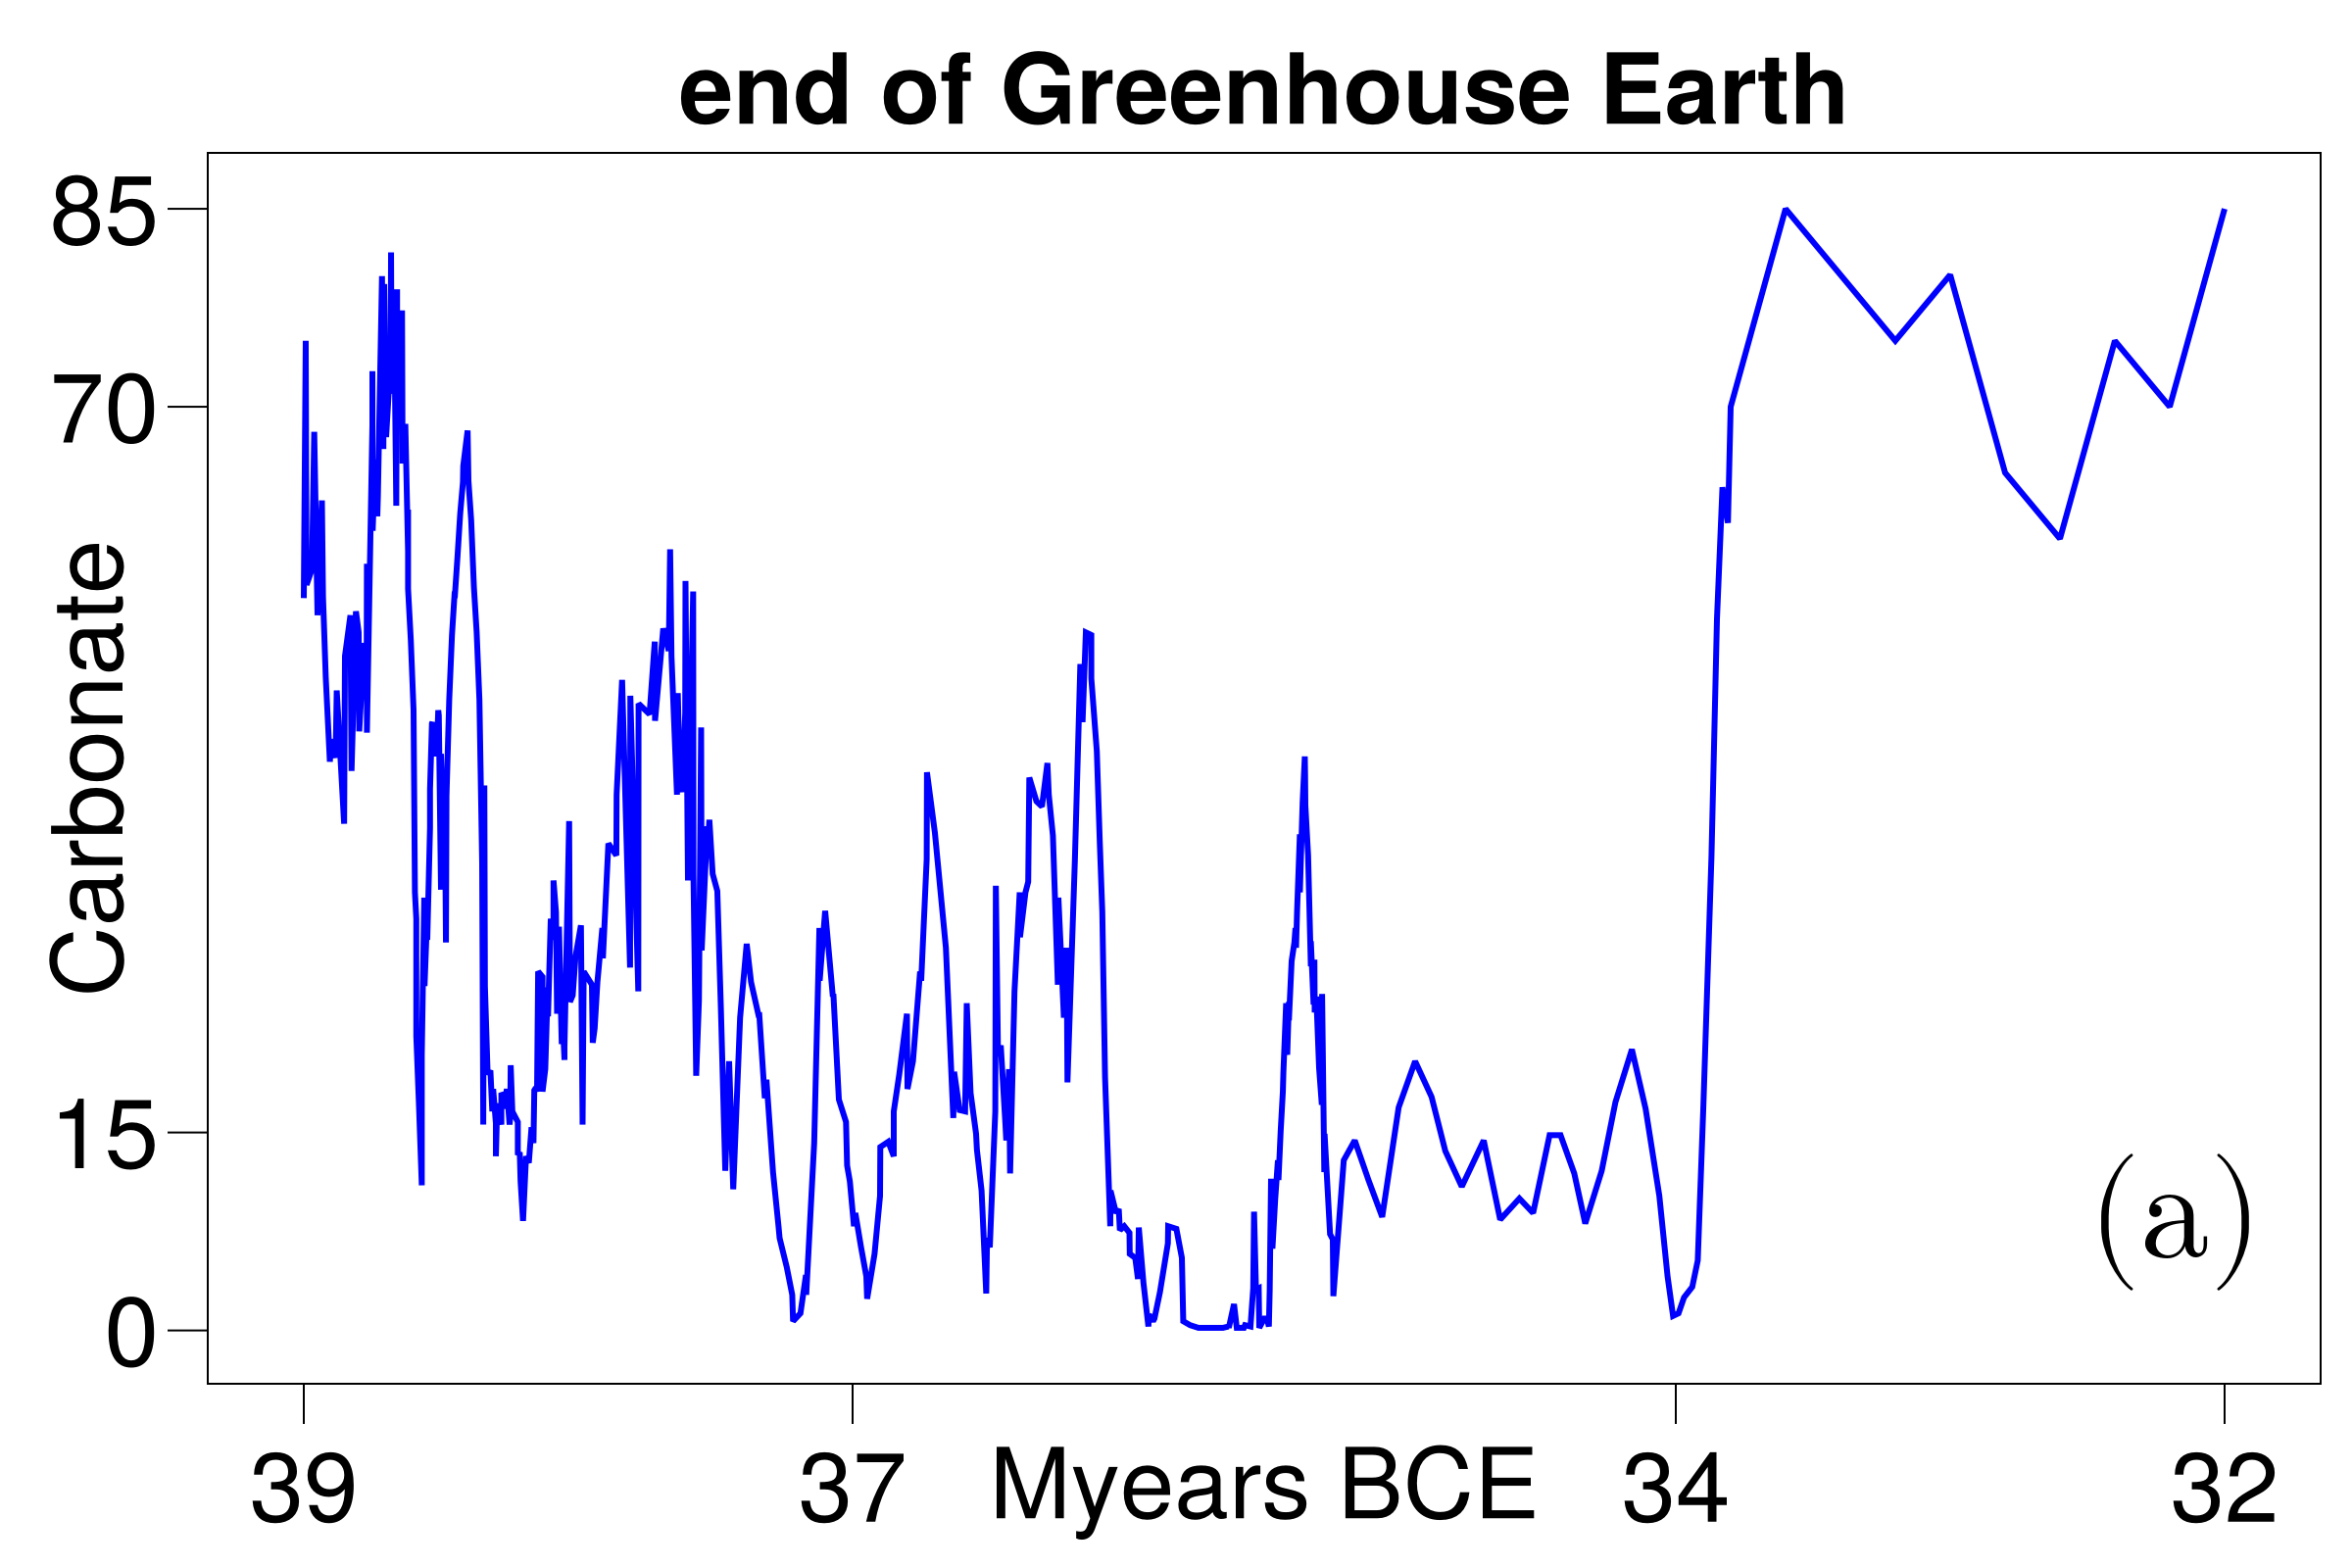
\includegraphics[keepaspectratio, width = \linewidth]{../figures/fig1.1.1.png}
        \label{fig1.1.1}
    \end{subfigure}
    \hfill
    \begin{subfigure}[b]{0.325\textwidth}
        \centering 
        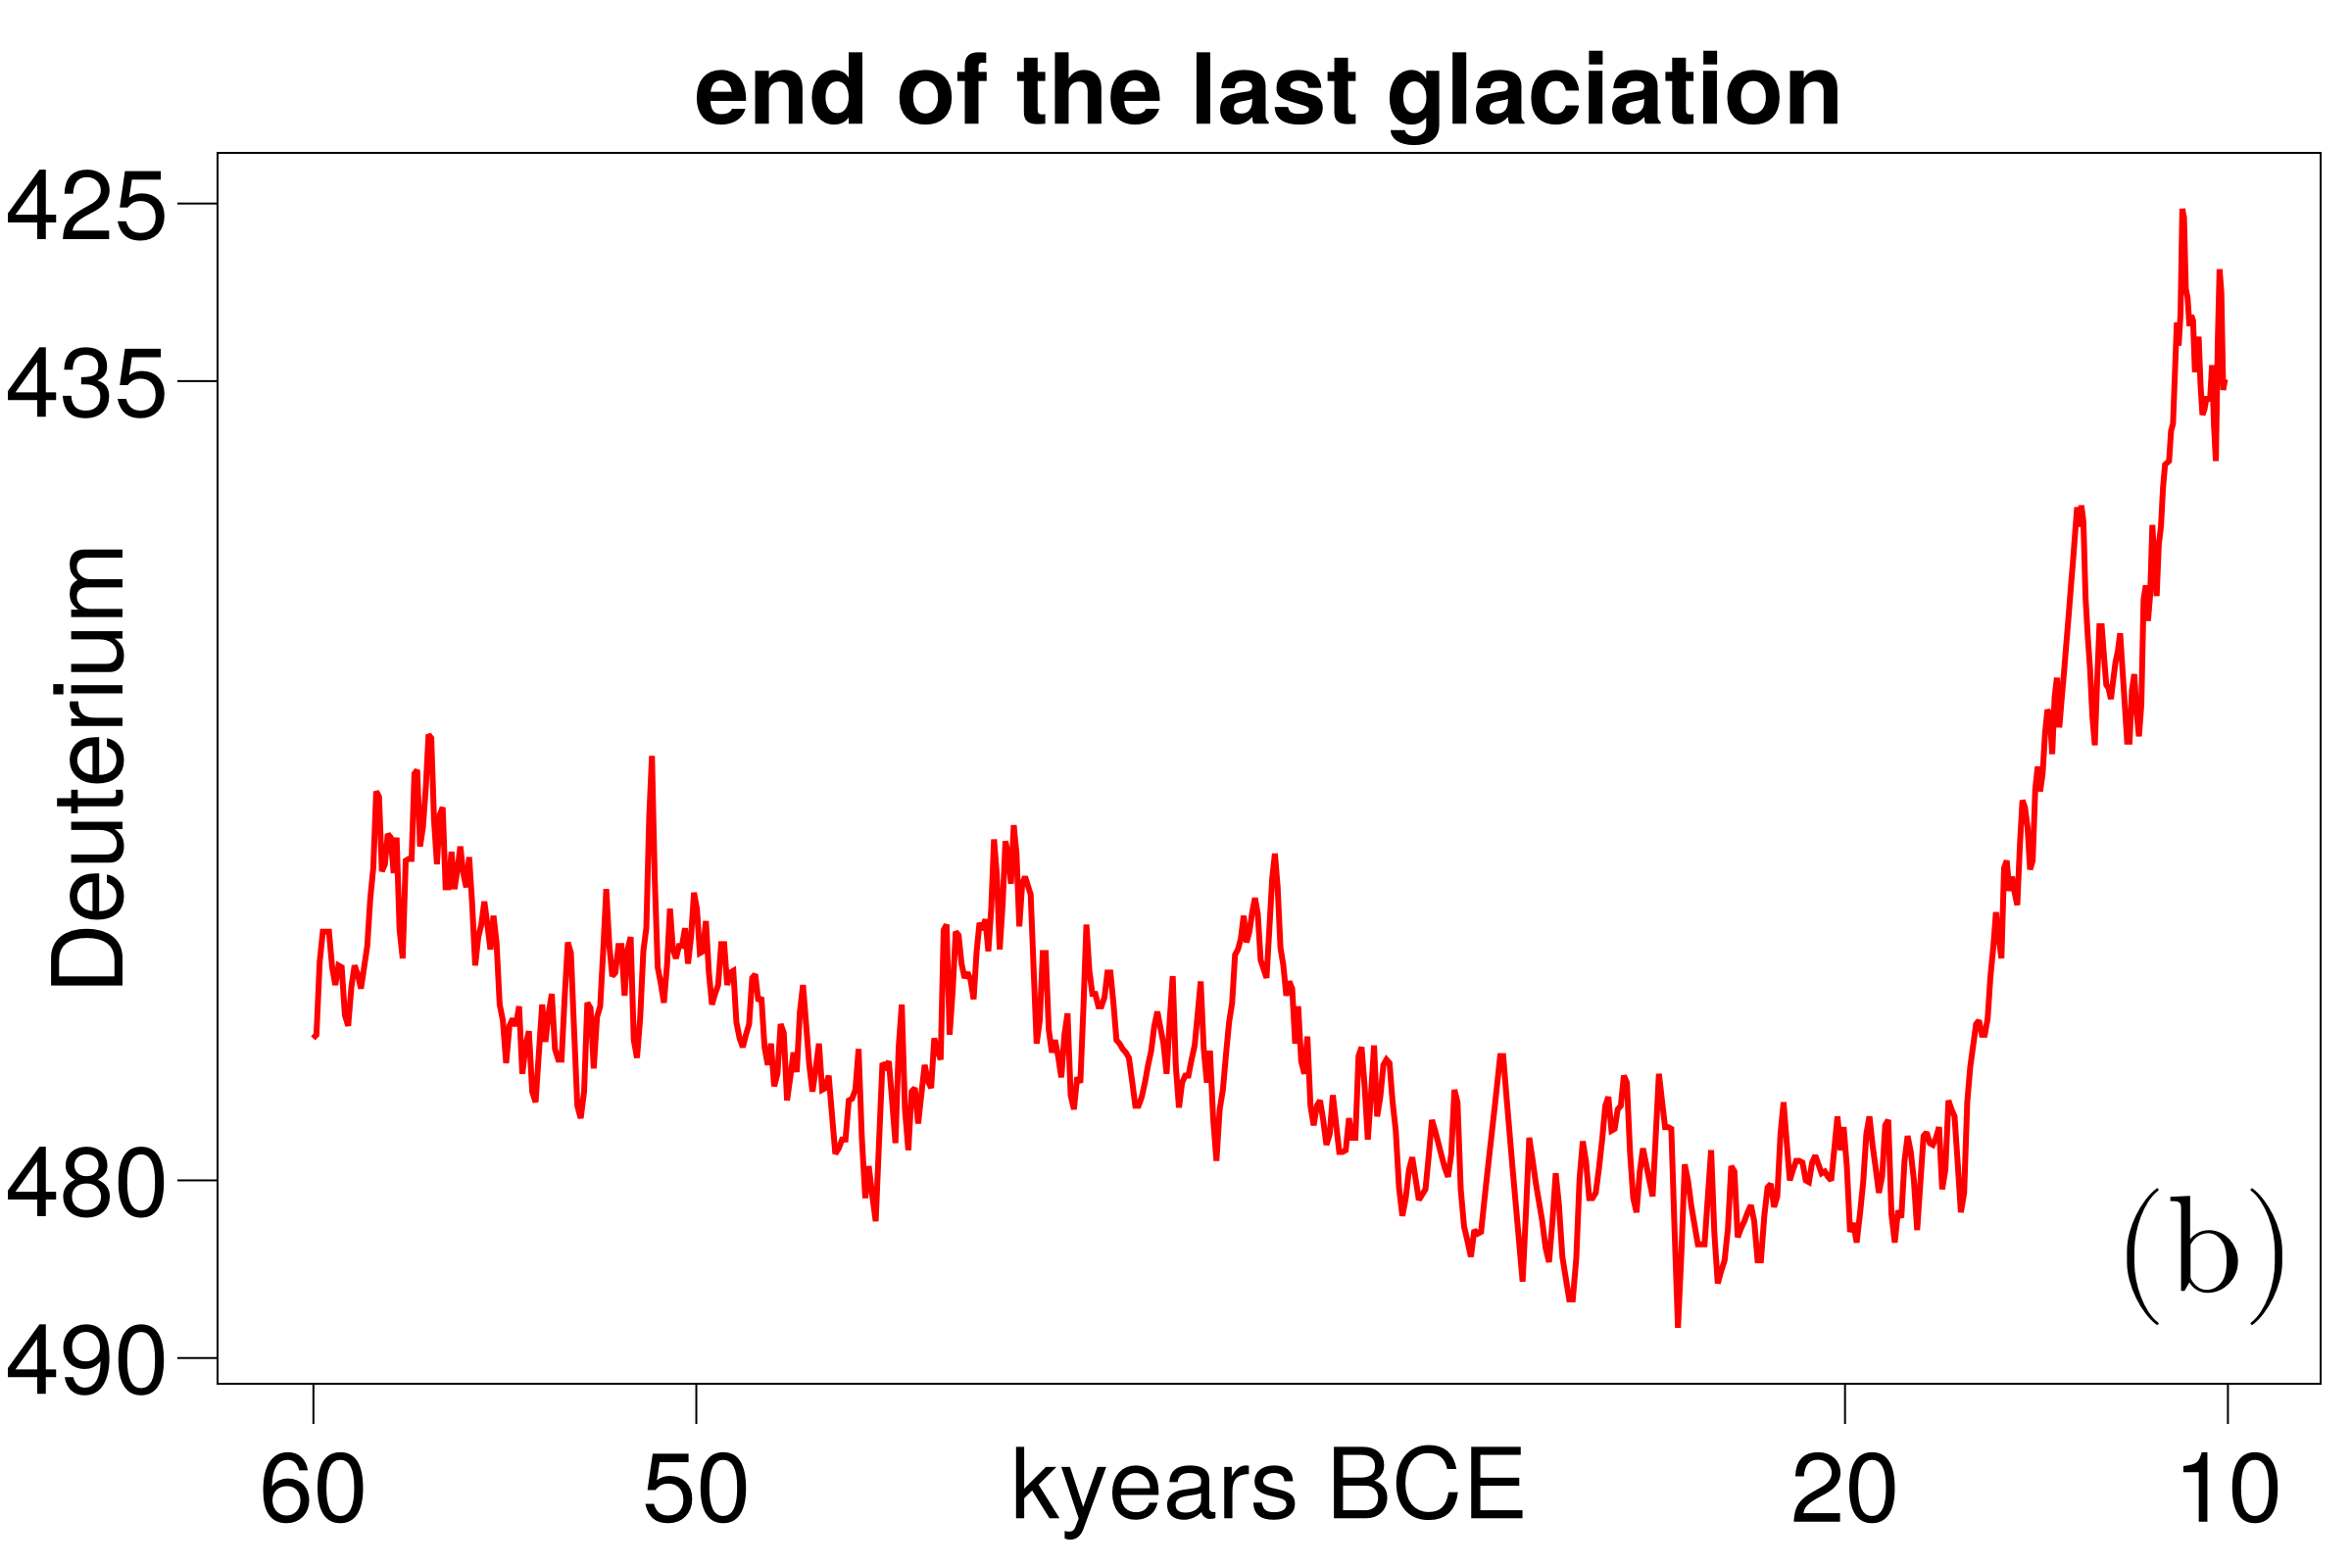
\includegraphics[keepaspectratio, width = \linewidth]{../figures/fig1.1.2.png}
        \label{fig1.1.2}
    \end{subfigure}
    \hfill
    \begin{subfigure}[b]{0.325\textwidth}
        \centering 
        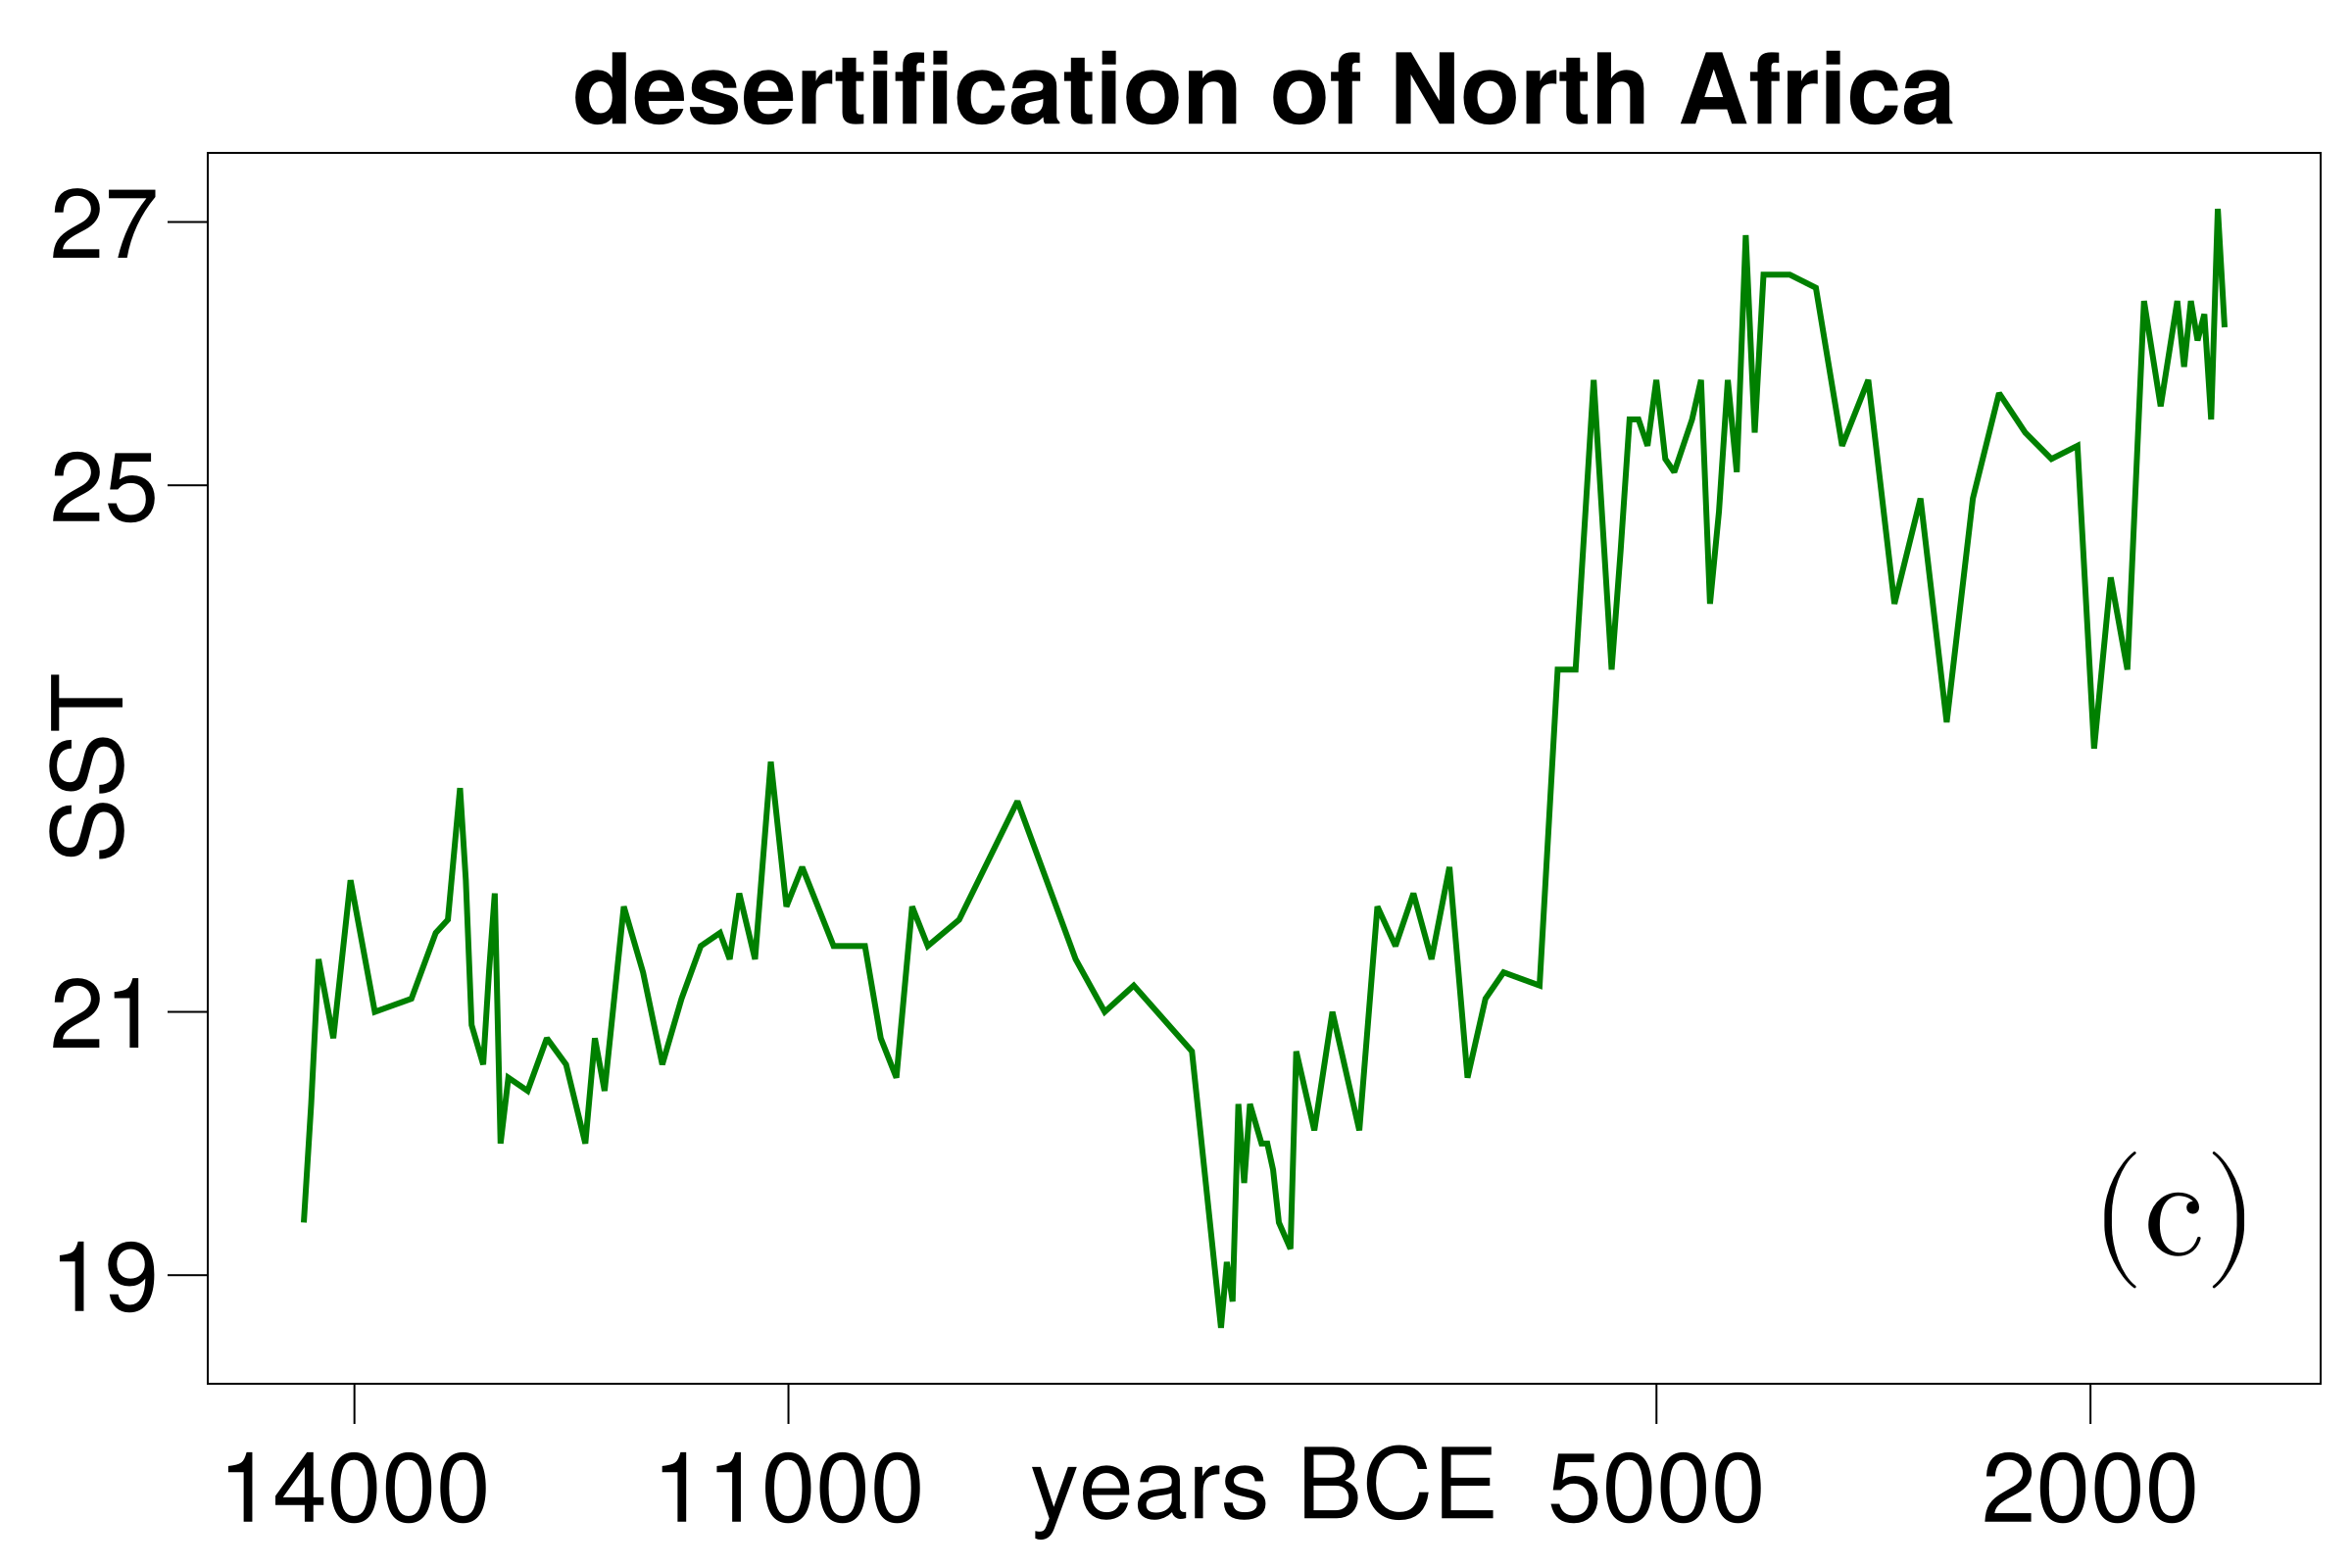
\includegraphics[keepaspectratio, width = \linewidth]{../figures/fig1.1.3.png}
        \label{fig1.1.3}
    \end{subfigure}


    \begin{subfigure}[b]{0.325\textwidth}
        \centering 
        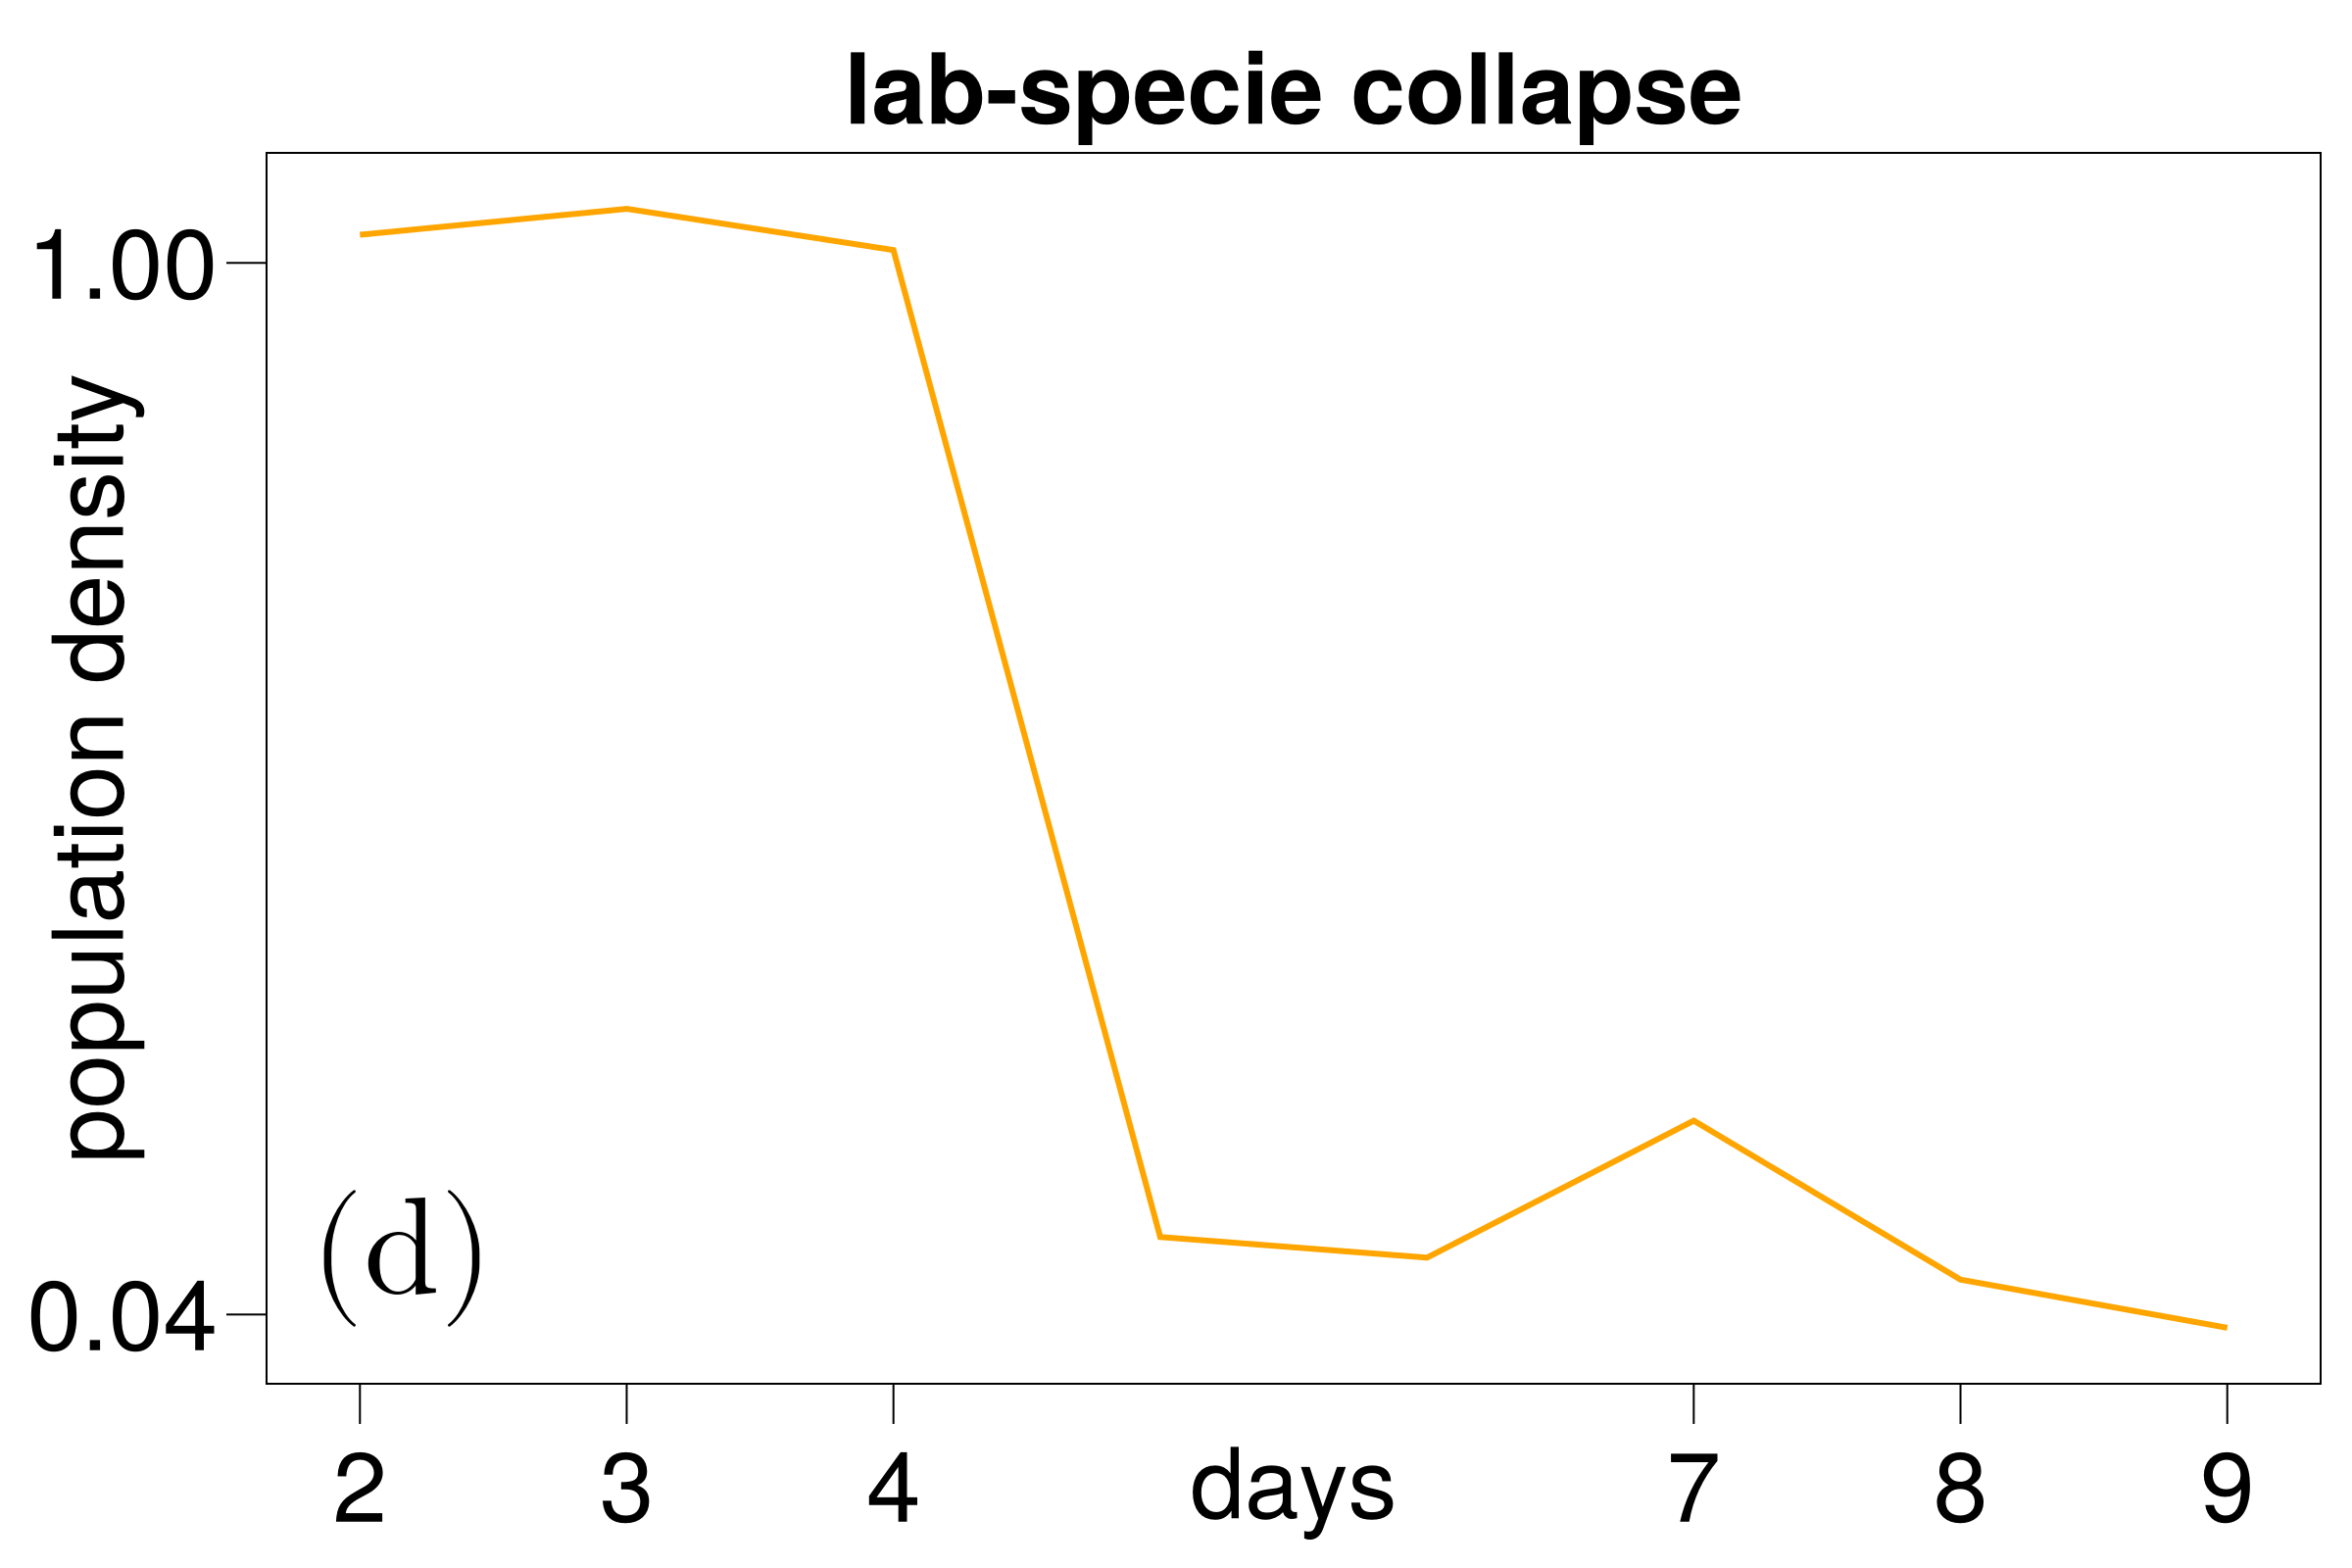
\includegraphics[keepaspectratio, width = \linewidth]{../figures/fig1.1.4.png}
        \label{fig1.1.4}
    \end{subfigure}
    \hfill
    \begin{subfigure}[b]{0.325\textwidth}
        \centering 
        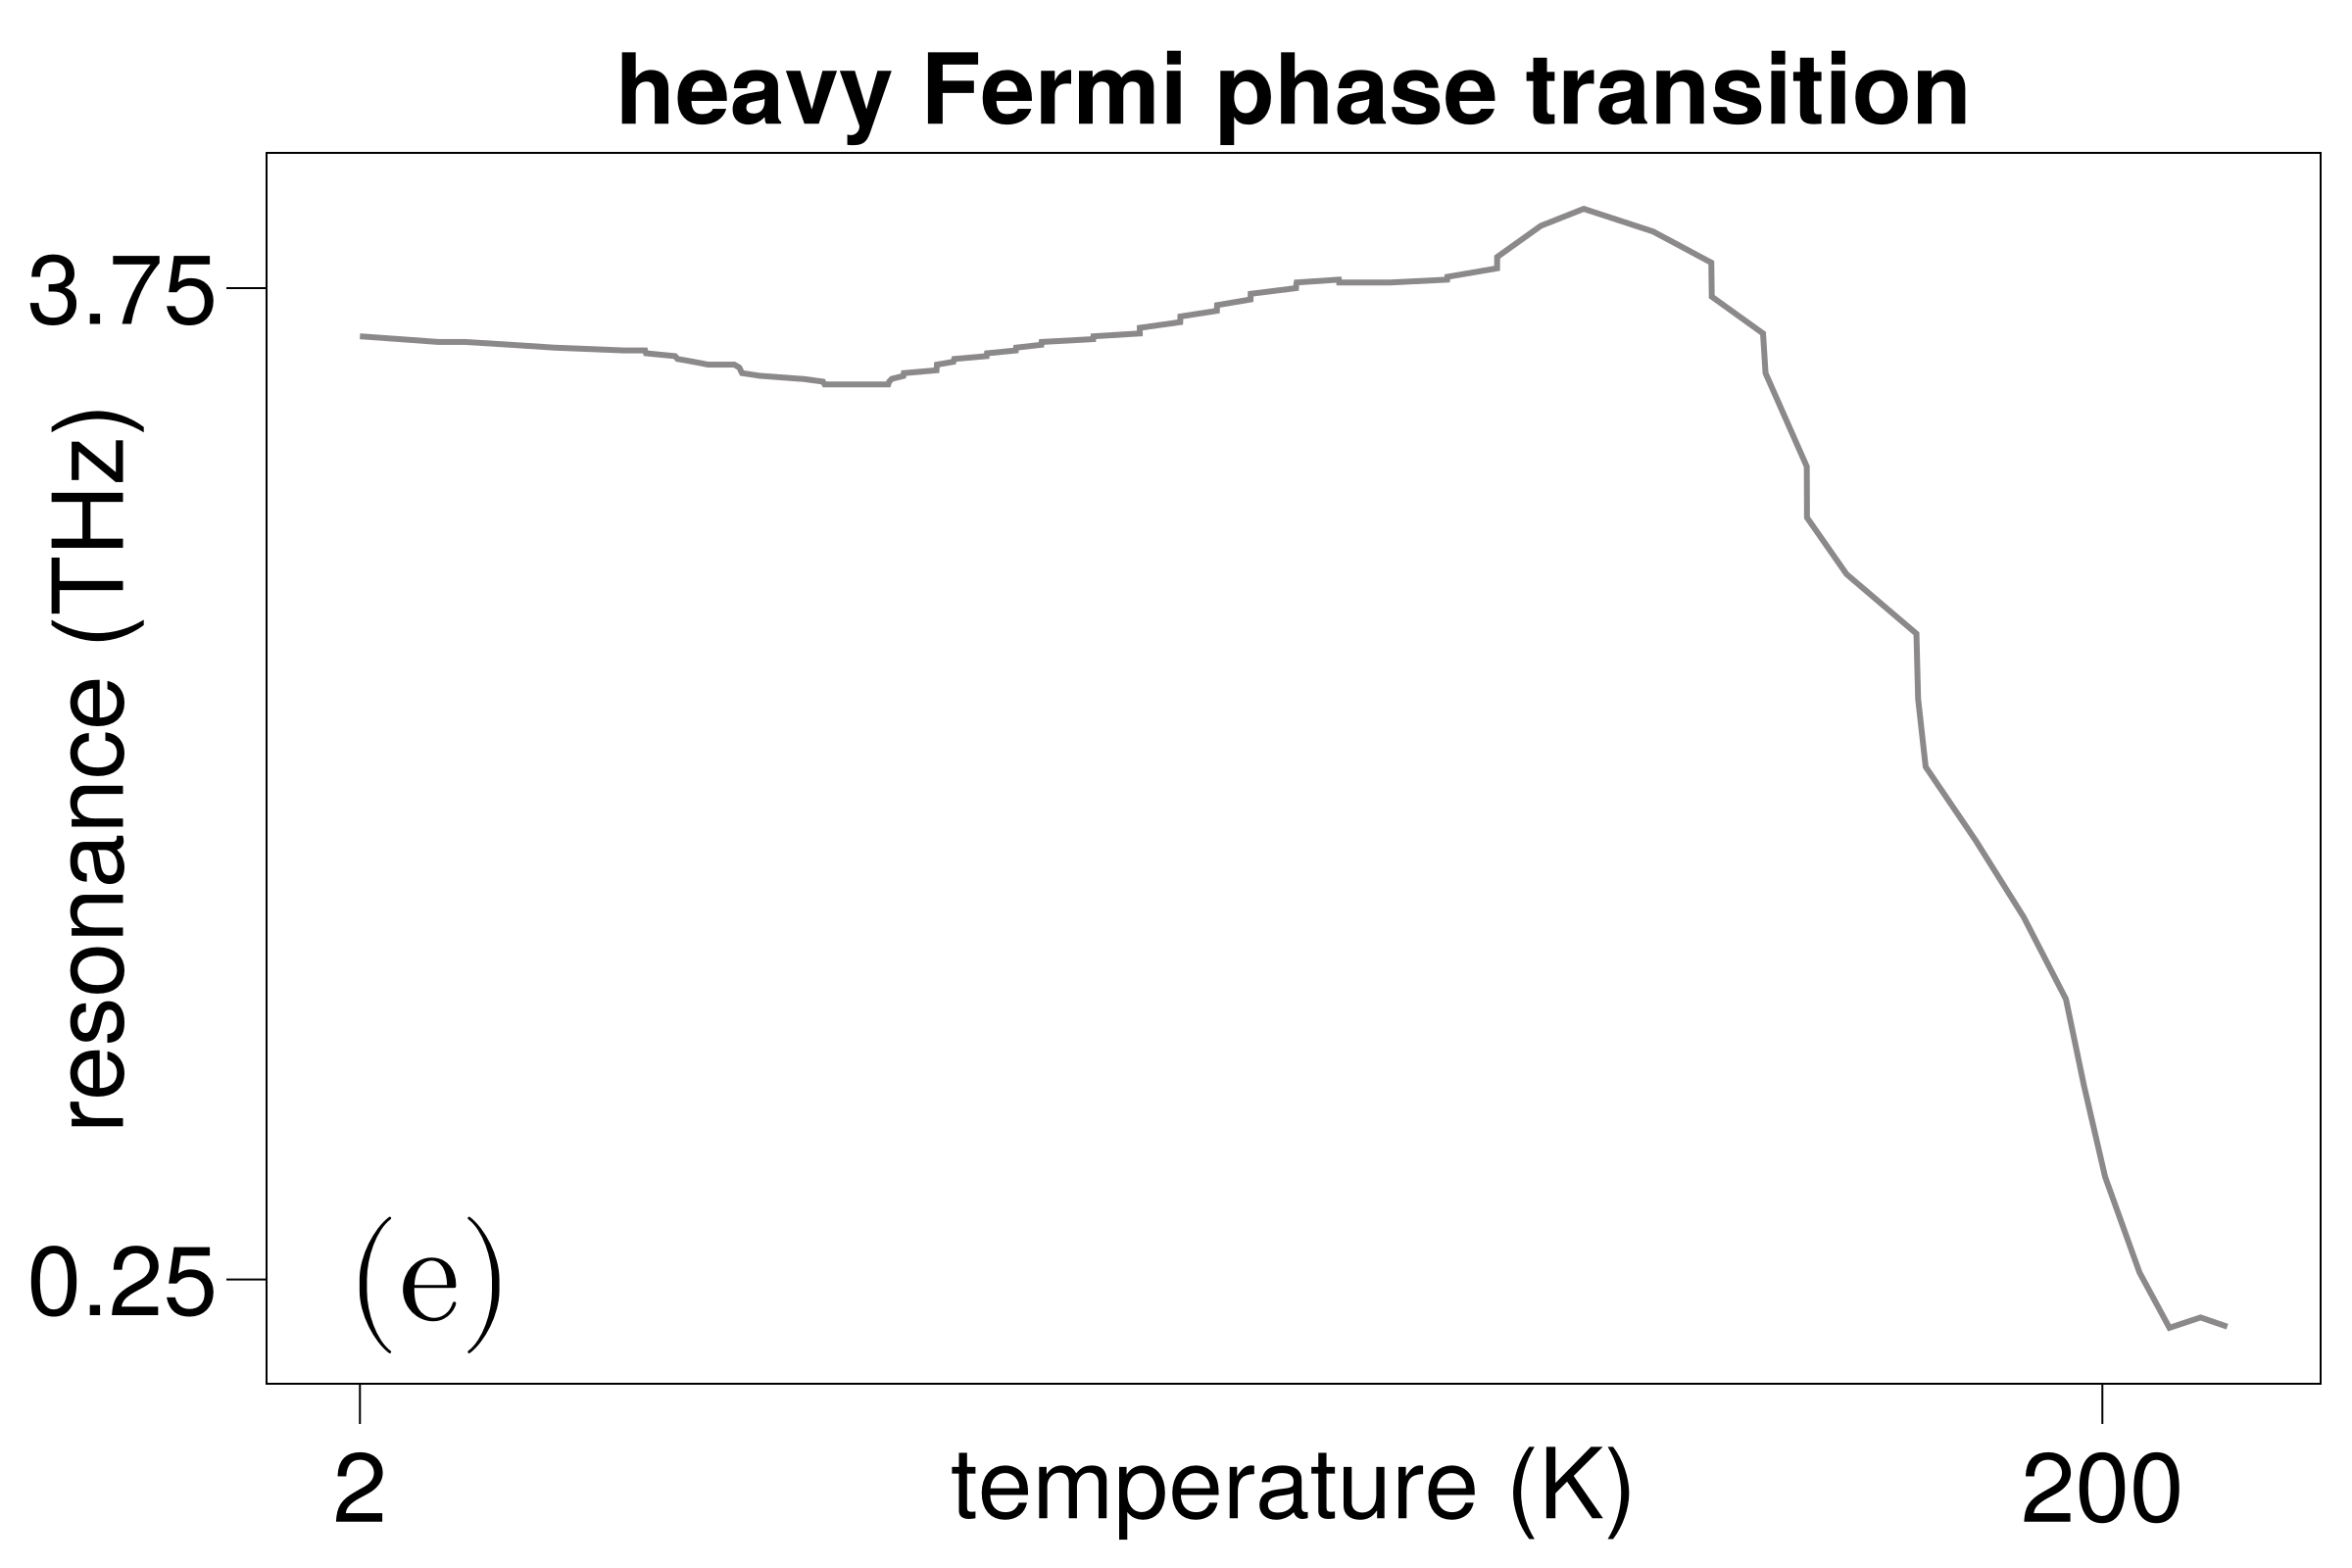
\includegraphics[keepaspectratio, width = \linewidth]{../figures/fig1.1.5.png}
        \label{fig1.1.5}
    \end{subfigure}
    \hfill
    \begin{subfigure}[b]{0.325\textwidth}
        \centering 
        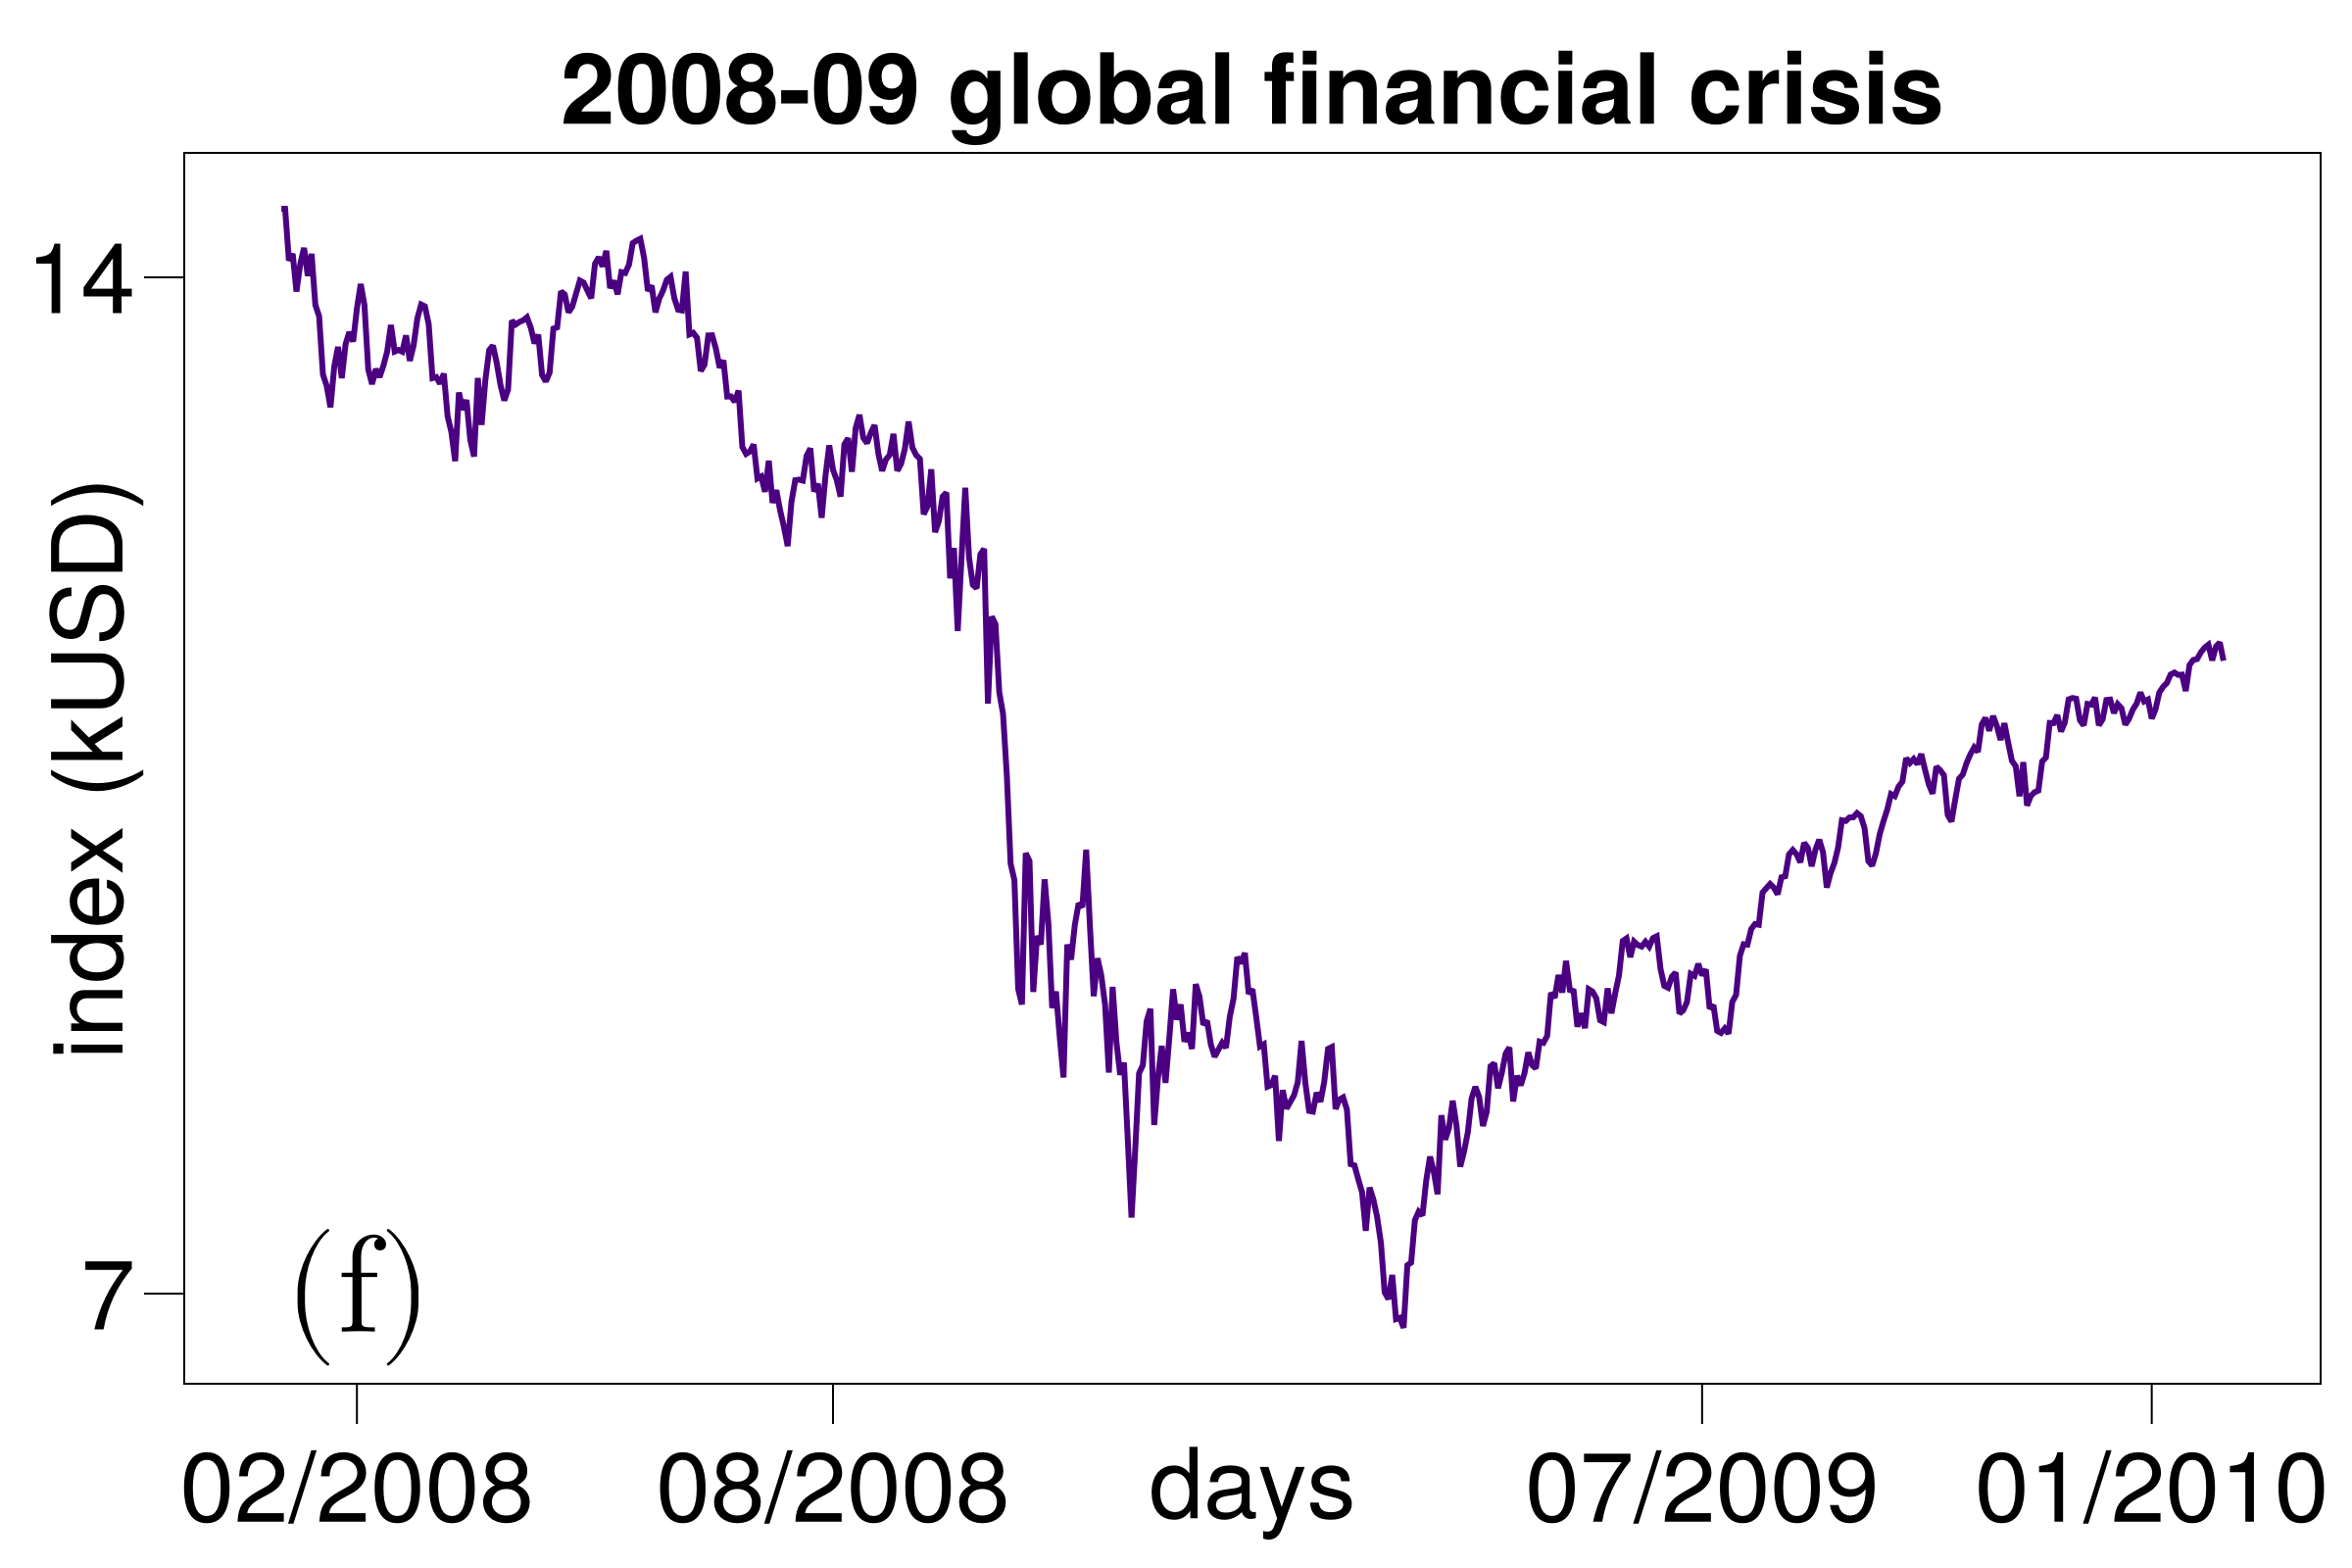
\includegraphics[keepaspectratio, width = \linewidth]{../figures/fig1.1.6.png}
        \label{fig1.1.6}
    \end{subfigure}
    \caption{Examples of real-world timeseries exhibiting a sudden regime shift (tipping event): (a) transition from Greenhouse to Icehouse Earth measured by calcium carbonate (CaCO$_3$) concentration in sediments of the tropical Pacific; (b) end of the last glacial period (LGP), colloquially referred to as the last ice age, detected as a transition of Deuterium ($2$H) concentrations in the ice core of Vostok, Antarctica; (c) abrupt end of the African humid period and onset of desertification from mean sea surface temperature (SST) measured in oceanic drilled holes off the cost of North-East Africa; (d) population collapse of a lab-grown ecosystem of budding yeast; (e) quantum phase transition from antiferromagnetic to heavy Fermi liquid of YbRh$_2$Si$_2$ measured as fermionic breakdown causing an abrupt decay of the resonant (spectroscopy) frequency; (f) global financial crisis caused by the collapse of subprime mortgages reflected by the Standard and Poor's 500 (S\&P 500) stock market index.
    Information about the sources of these study and the data points for the timeseries is provided in the Supplementary material.}
    \label{fig1.1}
\end{figure}
\subsection{Research context}\label{subsec1.2}
When considering EWS of critical transitions a distinction has to be made between the observed precursor, that is a phenomoenological pattern that the system exhibits as it approaches the threshold, and the indicator itself, which is a specific measurable signal that characterises the registered phenomenon.
This discernment is fundamental in the characterisation of EWS given by the fact that the same precursor can be measured by different indicators (see Table \ref{tab2.1}).
As an example consider \textit{critical slowing down} (CSD), arguably the most studied and well understood precursor in climate and ecological systems. 
It specifically refers to the observed behaviour of a dynamical system to become less resilient to perturbations of its stable equilibrium as a critical transition is approached. 
In other terms if the state of the system tracking an attractor comes close to a bifurcation then CSD is the symptomatic slower recovery towards the attractor w.r.t. small (noisy) perturbations.
This phenomenon can be measured in a variety of ways and thus a number of different indicators (both analytical and statistical) have been proposed throughout the years.
Other forms of precursors are \textit{flickering} and \textit{pattern-formation} and they also have been associated to the detection of multiple signals.
Some questions naturally arise following this separation, namely is there a better indicator than others for the clear and early detection of a critical transition? 
Is such indicator robust i.e. can it provide consistently a signal for the given precursor observed from different systems? 
Does it exist a universal measure that characterises critical transitions a-priori i.e. without prior knowledge of neither the presence of a bifurcation nor the functional model of reference?
Answers to these queries have been the subject of several efforts in the last 10 years and, to some extent, generic and robust indicators of abrupt regimes shifts have been achieved for a subset of simplified models.
For the rest of the present section we will outline a condensed but representative genealogy of EWS of critical transitions.
\subsubsection{Critical slowing down as loss of resilience}\label{subsubsec1.2.1}
Detection of early signs of incoming catastrophic events can take several forms. As mentioned above, the first occurence that was proposed as a precursor of such events is a phenomenon known as CSD.
The origin of the adoption of this term in dynamical systems can be traced back to 1994 Strogatz's seminal book \cite{Strogatz94} (which further mentions the name to be coined in statistical mechanics) and it referred to the lethargic (algebraic) decay of solutions to the stable equilibrium in the proximity of a supercritical pitchfork bifurcation (as opposed to the fast, exponential decay away from the bifurcation). 
\paragraph{1980s and 1990s}
This was proved mathematically one decade earlier in \cite{Wissel84} where it was shown how the return time of the system to its attractor depends on the inverse of the leading eigenvalue of the linearisation of the dynamics around the equilibrium.
As such attractor approaches a critical threshold it would thus exhibit infinitely slower return rate from a small perturbation.
As far as we know, the characteristic return time is the first indicator foretelling a critical transition.
The derivation of this \textit{``universal law"} was motivated by the study of thresholds of instabilities in multi-stable ecological systems \cite{May77} which in retrospective appears to be somehow prophetic of the communities that will extensively apply CSD forewarning catastrophic population collapses 2 decades later.
The influence of noise in such perturbations was characterised shortly thereafter in \cite{Wiesenfeld86} which linked the frequency range of the disturbance with the simplest codim$-1$ bifurcations showing that small-signal amplification was indeed a feature of these autonomous dynamical systems.
In 1995 this concept was (arguably independently) explored in \cite{Ives95} for stochastic dynamical systems. 
In there the \textit{resilience} of ecological systems was quantified statistically to be the ratio of the variability of population densities to variability in population growth rates. The study mentions the return time to equilibrium as the deterministic equivalent of stochastic resilience.
\begin{figure}[H]
    \centering 
    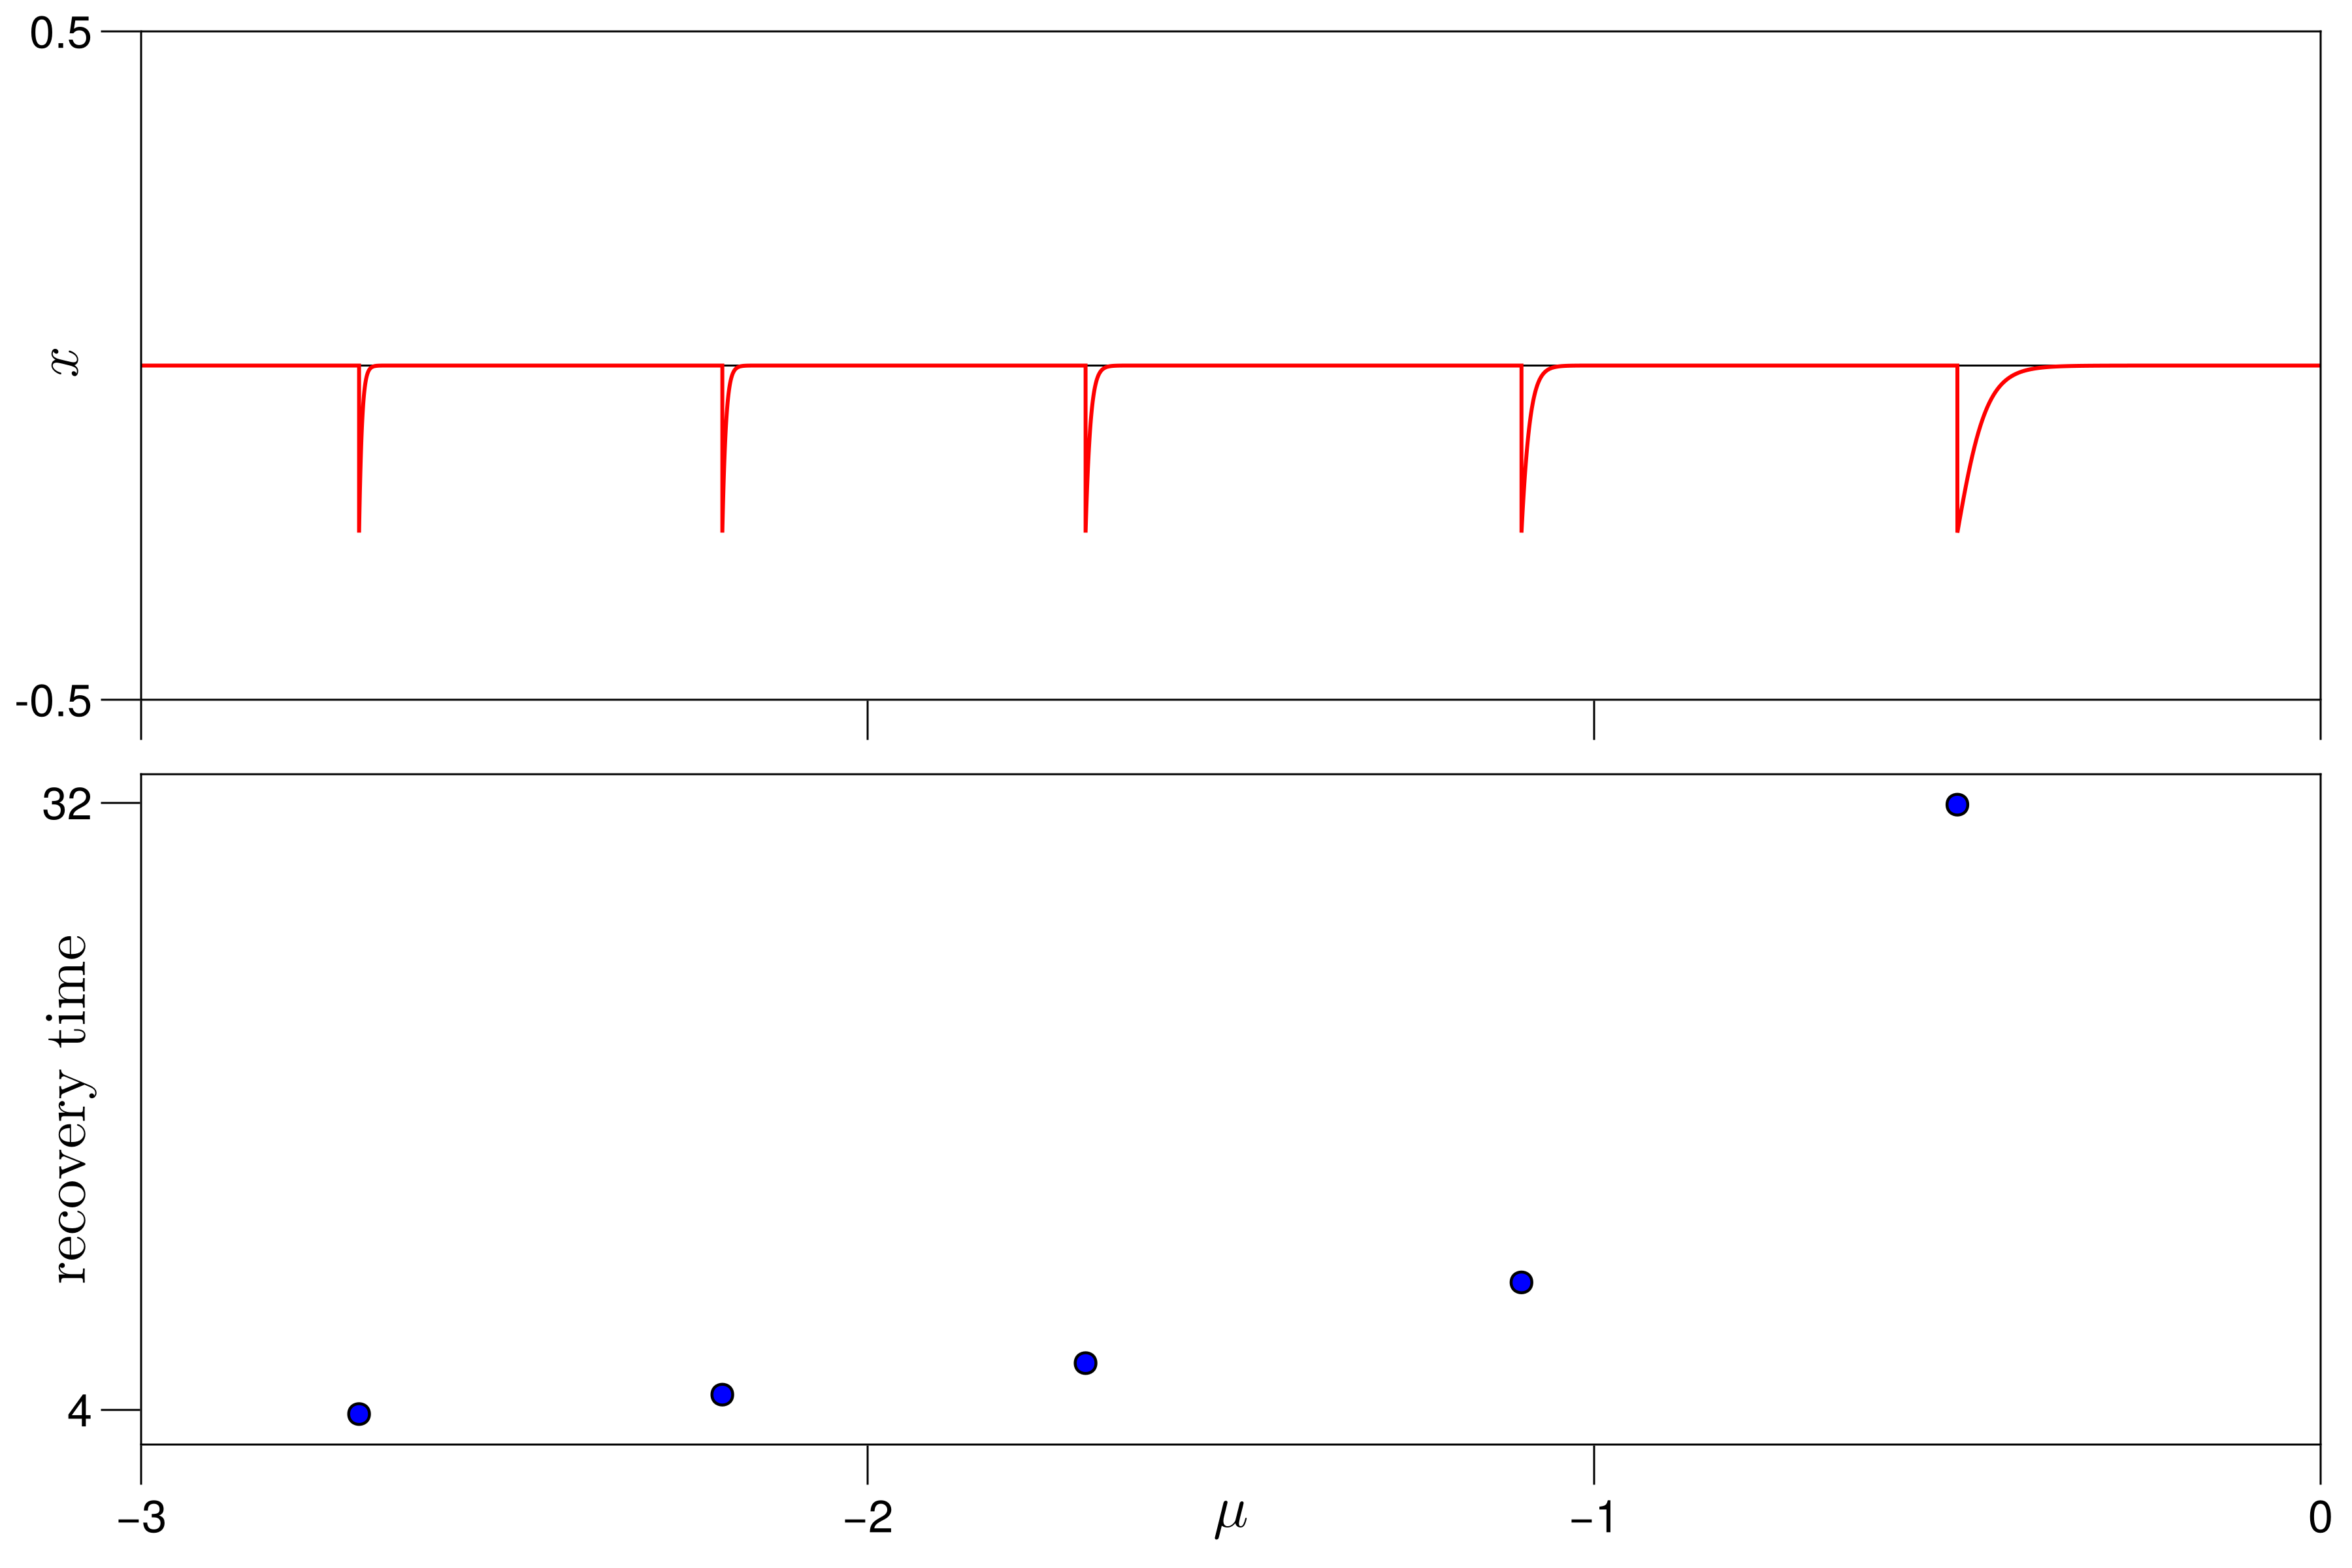
\includegraphics[keepaspectratio, width=\textwidth]{../figures/fig1.2.png}
    \caption{The phenomenon of CSD illustrated for a transcritical normal form. As the parameter approaches the bifurcation value $\mu=0$ small perturbations of the state (red line) tracking the attractor $x=0$ result in increasingly longer recovery. The return time is estimated numerically (blue dots) for each perturbation.}
    \label{fig1.2}
\end{figure}
It then took almost one decade to the ecologists to realise that, as catastrophic switches between stable population's states occurred unannounced when one only monitors the state variables (as for a saddle-node bifurcation \cite{Scheffer01}) the derivation of EWS was necessary to predict these disruptive shifts and act upon the external forcing to prevent them. 
\paragraph{Mid 2000s}
In 2005 it was observed \cite{Oborny05} that the spatial dynamics of a logistic model organised on a square lattice exhibits fractal-like subdivisions of the competing species and suggested that the scaling law of the spatial variance near the extinction can be used as a EWS. 
It was one year later when Carpenter and Brock \cite{Carpenter06} formalised this idea and conjectured how increases in the variance of the timeseries of a stochastic differential equation (SDE) can be a clue of impending regime shifts.
The rise in variance of SDEs as an indicator of CSD will not be rigorously proved mathematically for another 5 years when Kuehn \cite{Kuehn11} formalised it in the framework of fast-slow dynamics (discussed later in Section \ref{subsubsec2.1.3}).
Nevertheless there is a pleasant intuition for this measure of CSD as discussed in \cite{Scheffer09}. 
As CSD is associated to a slower recovery from forced perturbations, due to the leading eigenvalue of the respective Jacobian approaching the immaginary axis, the intrinsic rate of change of the realizations of the SDE diminishes. 
This in turn is reflected in the timeseries to exhibit memory of its past i.e. the state at the next iteration will be somewhat related to some order of its past states. 
This intuition is already enough to suggest the autocorrelation of lagging order $p$ (AC($p$)) to be an indicator of CSD.
However if one is willing to force some form of equivalence between a more sluggish timeseries w.r.t. perturbations and a random walk (which has a monotonic trend in variance depending linearly on time) then rise in the variance can be reasonably assumed as an EWS of an upcoming bifurcation.
Perhaps the major significance of Carpenter's and Brock's 2006 paper for the ecology community was the suggested implication that, by relying merely on timeseries data, a catastrophic population collapse can be predicted early enough even without knowing the underlying model (or assuming high levels of uncertainties in the estimation of parameters and noise levels). 
Prior to their proposal however, earlier works in the climate community proposed different types of indicators for estimating the distance to bifurcations of the North Atlantic thermoaline circulation (THC) under (stochastic) freshwater forcing driven by climate change. 
In particular in 2003 a simplified box model of the THC was deployed to estimate (analytically) the dependence of shifts in the frequency spectrum of the idealised Ornstein-Uhlenbeck process (OUP) of the deviations of the salinity gradient from equilibrium to the (bi-stable) saddle-node bifurcation in the model \cite{Kleinen03} (which became known as spectral reddening).
One year later the same first author also co-authored an investigation for larger, more realistic models of the THC in a numerical setting \cite{Held04} and concluded that an increased variability is a better diagnostic tool at anticipating the overturning circulation.
These works spurred a vast uptake by climate scientist and ecologist in the role of CSD and in general in the potential of statistical measures that are prognostics of catastrophic regime shifts in their respective systems.
\subsubsection{Criticism of EWS from climate and ecosystem timeseries}\label{subsubsec1.2.2}
A substantial wealth of works was published in the following decade marking the beginning of intense research and categorisation of EWS from a dynamic perspective. 
We can think of the years spanning from 2007 to 2015 as the \textit{gold rush} era of EWS in climate and ecology.
\paragraph{Late 2000s}
Regarding the former, in 2007 a method based on detrended fluctuation analysis (DFA) was introduced by Livina and Lenton \cite{Livina07} to improve upon the estimation of the decay rate, and hence the proximity to a climate bifurcation, from paleoclimate records. 
They realised that the non-stationarity of (climate) timeseries approaching a bifurcation somehow pollute the statistical scaling properties used to estimate the non-linear shifts. 
The importance of detrending dynamical timeseries will be made clear in the third Chapter of the present work.
In the same year van Nes and Scheffer \cite{vanNes07} took note of this and explored the estimation of the recovery rate from perturbations by fitting an exponential process to the timeseries generated by $6$ simple, $1-$dimensional models of ecosystems. 
They also curcially mentioned the potential detection of \textit{false positives} and \textit{false negatives}.
This crossover between the two communities eventually led to the 2008 pivotal work by Dakos, Scheffer, van Nes et al. \cite{Dakos08} in which the first coefficient of a fitted autoregressive AR(1) model (which measures the autocorrelation at lag-1) was shown to consistently predict the onset of critical transitions in $8$ major paleoclimate events ($3$ of which are reported in Figures \ref{fig1.1}(a)-\ref{fig1.1}(c) above), i.e. using real-world data rather than model-based simulations.
In the following 3 years several forms of indicators prognostic of CSD were proposed and applied to different population models. 
We mention, among others: kurtosis and skewness \cite{Biggs09} used in a fisheries food web model (which found weaker signals compared to AR(1) and reddening of the spectral density ratio); the analytical recovery rate of Hopf and transcritical bifurcations of the $2-$dimensional predatory-prey and Lotka-Volterra models \cite{Chisholm09}; variance, autocorrelation and skewness in the transcritical bifurcation of an experimental population in a deteriorating environment \cite{Drake10}; variance, return rate, skewness and spectral ratio in a monitored lake ecosystem \cite{Carpenter11a}; the total variance of a fitted drift-diffusion-jump (DDJ) model \cite{Carpenter11b} for non-parametric, data-generating processes.
Soon after reviews of EWS of critical transitions became available, most notably Scheffer, Carpenter, Dakos et al. \cite{Scheffer09} and Lenton \cite{Lenton11}. In 2009 Scheffer also published a book \cite{Scheffer09b} on critical transitions compiled until then in natural and human sciences.
\paragraph{Early 2010s}
With this new discipline gaining traction it also, naturally, attracted some criticism. 
In 1977 the implications of catastrophic events in biological and social sciences was put in question \cite{Zahler77} by \textit{``incorrect reasoning"} and \textit{``far-fetched assumptions"} regarding cusp bifurcations.
With regards to the robustness of the statistical indicators a more recent work in 2010 \cite{Ditlevsen10} argued that not all paleoclimate records show critical transitions due to bifurcation and are rather caused by stochastic fluctuations (known today as N-tippings, see Section \ref{subsec2.1}) which have very limited predictibility. 
The authors noted that by assessing the statistical significance of the variance and autocorrelation of records of the Dansgaard-Oeschger events (analysed by the ice core data in the North Greenland ice core project, or NGRIP) one showed a monotonic trend while the other showed no signal. 
This, the authors argued, was evidence that no bifurcation was approached by the system which instead tipped over to an alternative stable regime driven by noise alone, which is contrary to what was claimed in previous works \cite{Dakos08,Scheffer09}.
In addition, the same year, another work showed that abrupt population shifts in particular ecosystems (specifically when the magnitude of the stochastic fluctuations increases, i.e. higher noise levels) occured without forewarning \cite{Hastings10} of CSD (i.e. false negatives or \textit{missed alarms}).
The mathematical basis of the authors was that all the previous works showed EWS for (simplified) systems that have a smooth dependence of the potential landscape on the underlying parameter and did not consider real, complex systems exhibiting, for example, chaotic attractors. 
Ensemble simultations of the Ricker map did in fact lead to a failure of the aforementioned EWS in detecting the population collapse.
Increasing evidence supporting the lack of consistency of the proposed indicators was further provided in 2013 by Dakos, Scheffer et al. \cite{Kefi13} and others \cite{Boerlijst13}. 
In particular the latter followed the examples laid out in the previous papers, i.e. providing evidence of \textit{silent catastrophes} while the former went in the opposite direction and reported that variance and autocorrelation give a trend even for non-catastrophic events (i.e. false positives).
These $4$ works pointed out the urgency of: 
\begin{enumerate}
     \item a robust characterisation (in terms of statistical significance and some form of universality across different complex systems) of EWS;
     \item a deeper (and desirably rigorous) understanding of the mathematical structure of the analysis motivating the existence of EWS.
\end{enumerate}
The second of those two needs begun to be investigated by Kuehn in 2011 \cite{Kuehn11} and we discuss it in the next Chapter (see Sections \ref{subsubsec2.1.1} and \ref{subsubsec2.1.3}). The questions regarding the robustness and universality of the leading indicators of CSD also started to be addressed shortly thereafter and we will explore them further ahead (see Sections \ref{subsec2.3} and \ref{subsec3.1}).
\subsubsection{Flickering as an alternative sign of critical thresholds}\label{subsubsec1.2.3}
Contemporary to the rise of indicators for CSD and their critics, another phenomenon was being observed to be a precursor of regime shifts. We mentioned above some indicators s.a. increase in variance and skewness to be prognostic of CSD albeit showing weaker signals w.r.t. autocorrelation \cite{Biggs09,Drake10,Carpenter11a}.
Changing skewness in the distribution of the realizations of the timeseries was first proposed in 2008 \cite{Guttal08} as an indicator of increasing asymmetry in a number of simulated ecosystems. 
In such paper the origin of a trend in skewness as the models approached a critical transition was linked to the asymmetric change of the potential landscape of the SDE.
This prescribes that the state of the system has particular directions, towards which it may tip to, that are more favourable than others.
This observation is considerably different from the flattening of the potential landscape that is found at the core of CSD and as such suggested that a novel precursor was being measured by the proposed EWS.
This new phenomenon (it was shown) did not rely on the linearisation of the dynamics around the stable equilibrium and instead considered the effects of high noise levels to be dominant close to the critical threshold where alternative attractors became \textit{``available"} to the system under large fluctuations.
It would be thus reasonable to expect that systems that do not feature such asymmetry in the presence of multi-stable states will not exhibit stronger signals than those that are instead purely associated to the flattening of the potential landscape as prescribed by CSD.
\paragraph{Mid 2010s}
In 2010 this intuition was further validated by approximating the shape of the potential function (and thus estimating the number of states available to the system at given parameter values) by polynomial fitting of the empirical distribution of timeseries data \cite{Livina10}. 
The method, termed potential analysis, succesfully detected an increased number of alternative stable states for ice-core proxy records of paleotemperature transitions at NGRIP, thus providing yet another indicator of asymetric changes in the potential landscape of a model. 
Similarly to the increase in skewness, also the increase in variance, previously linked to CSD, was discovered to occur in unsteady excursions of the state towards alternate basins of attraction. Brock and Carpenter \cite{Brock10} thus distinguished the two sources of increased variance in the already known CSD and the new phenomenon which they named flickering. 
\begin{figure}[H]
   \begin{subfigure}[b]{0.475\textwidth}
        \centering 
        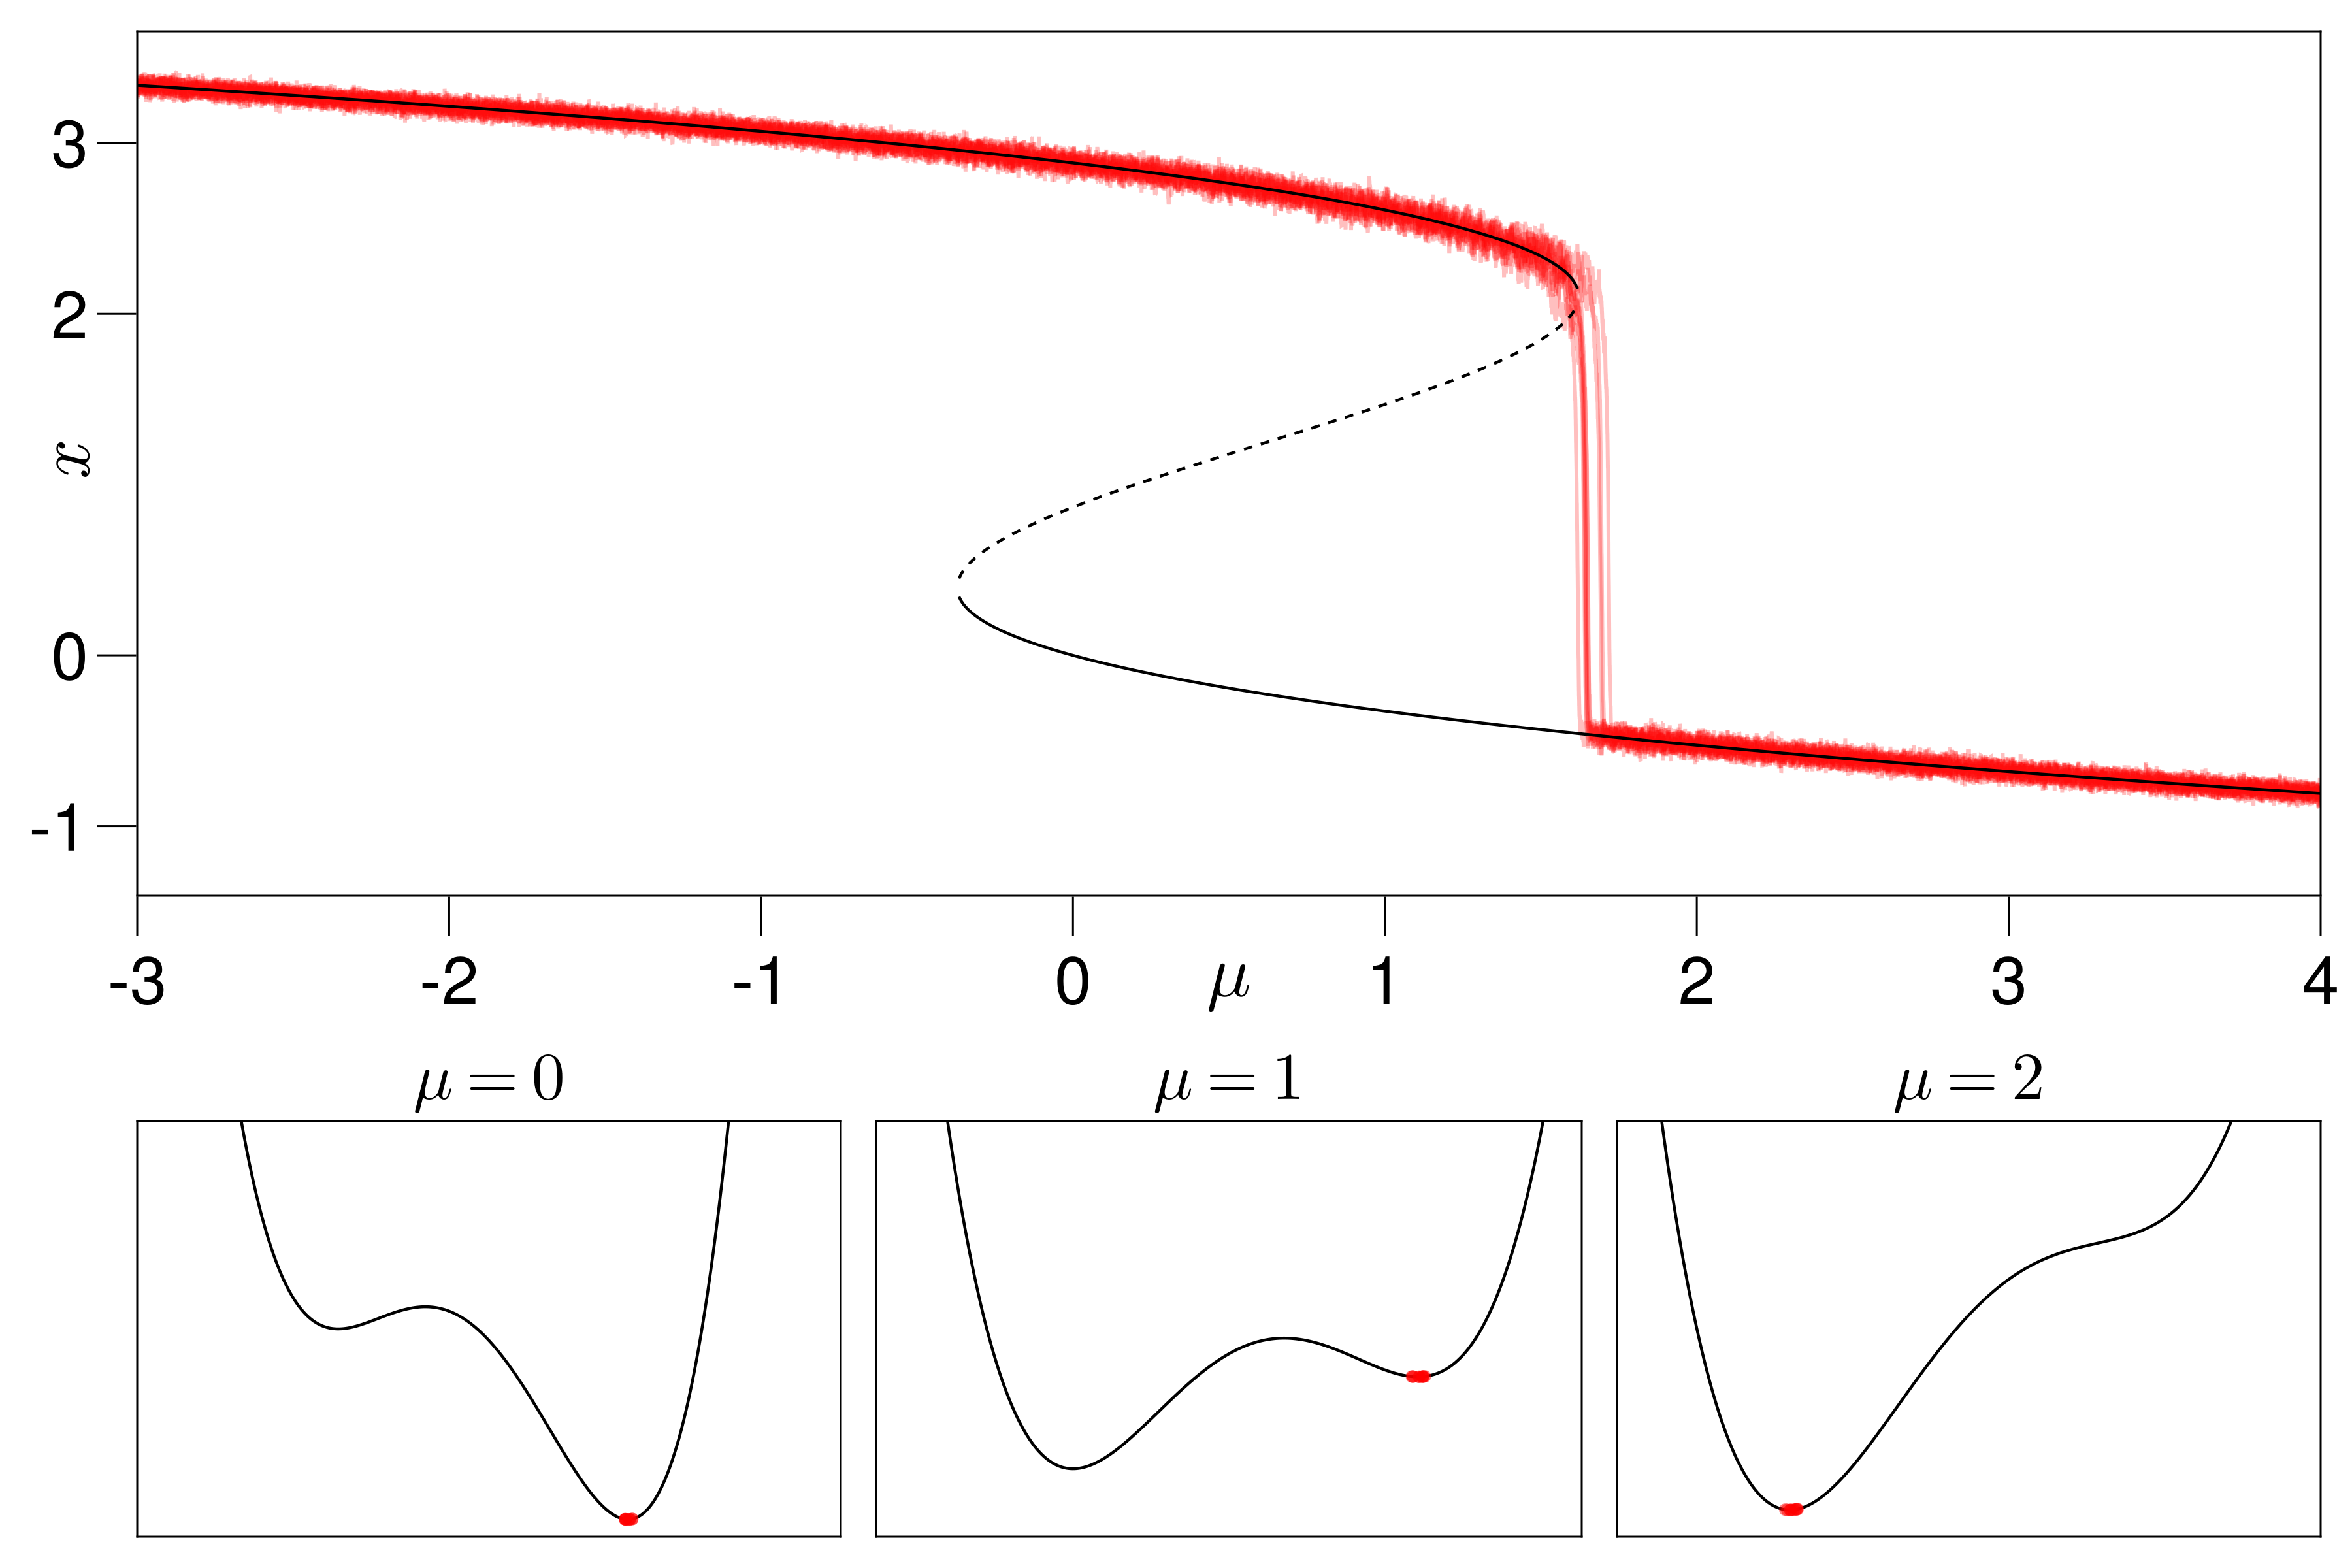
\includegraphics[keepaspectratio, width = \linewidth]{../figures/fig1.3.1.png}
        \caption{}
        \label{fig1.3.1}
   \end{subfigure}
   \hfill
   \begin{subfigure}[b]{0.475\textwidth}
        \centering 
        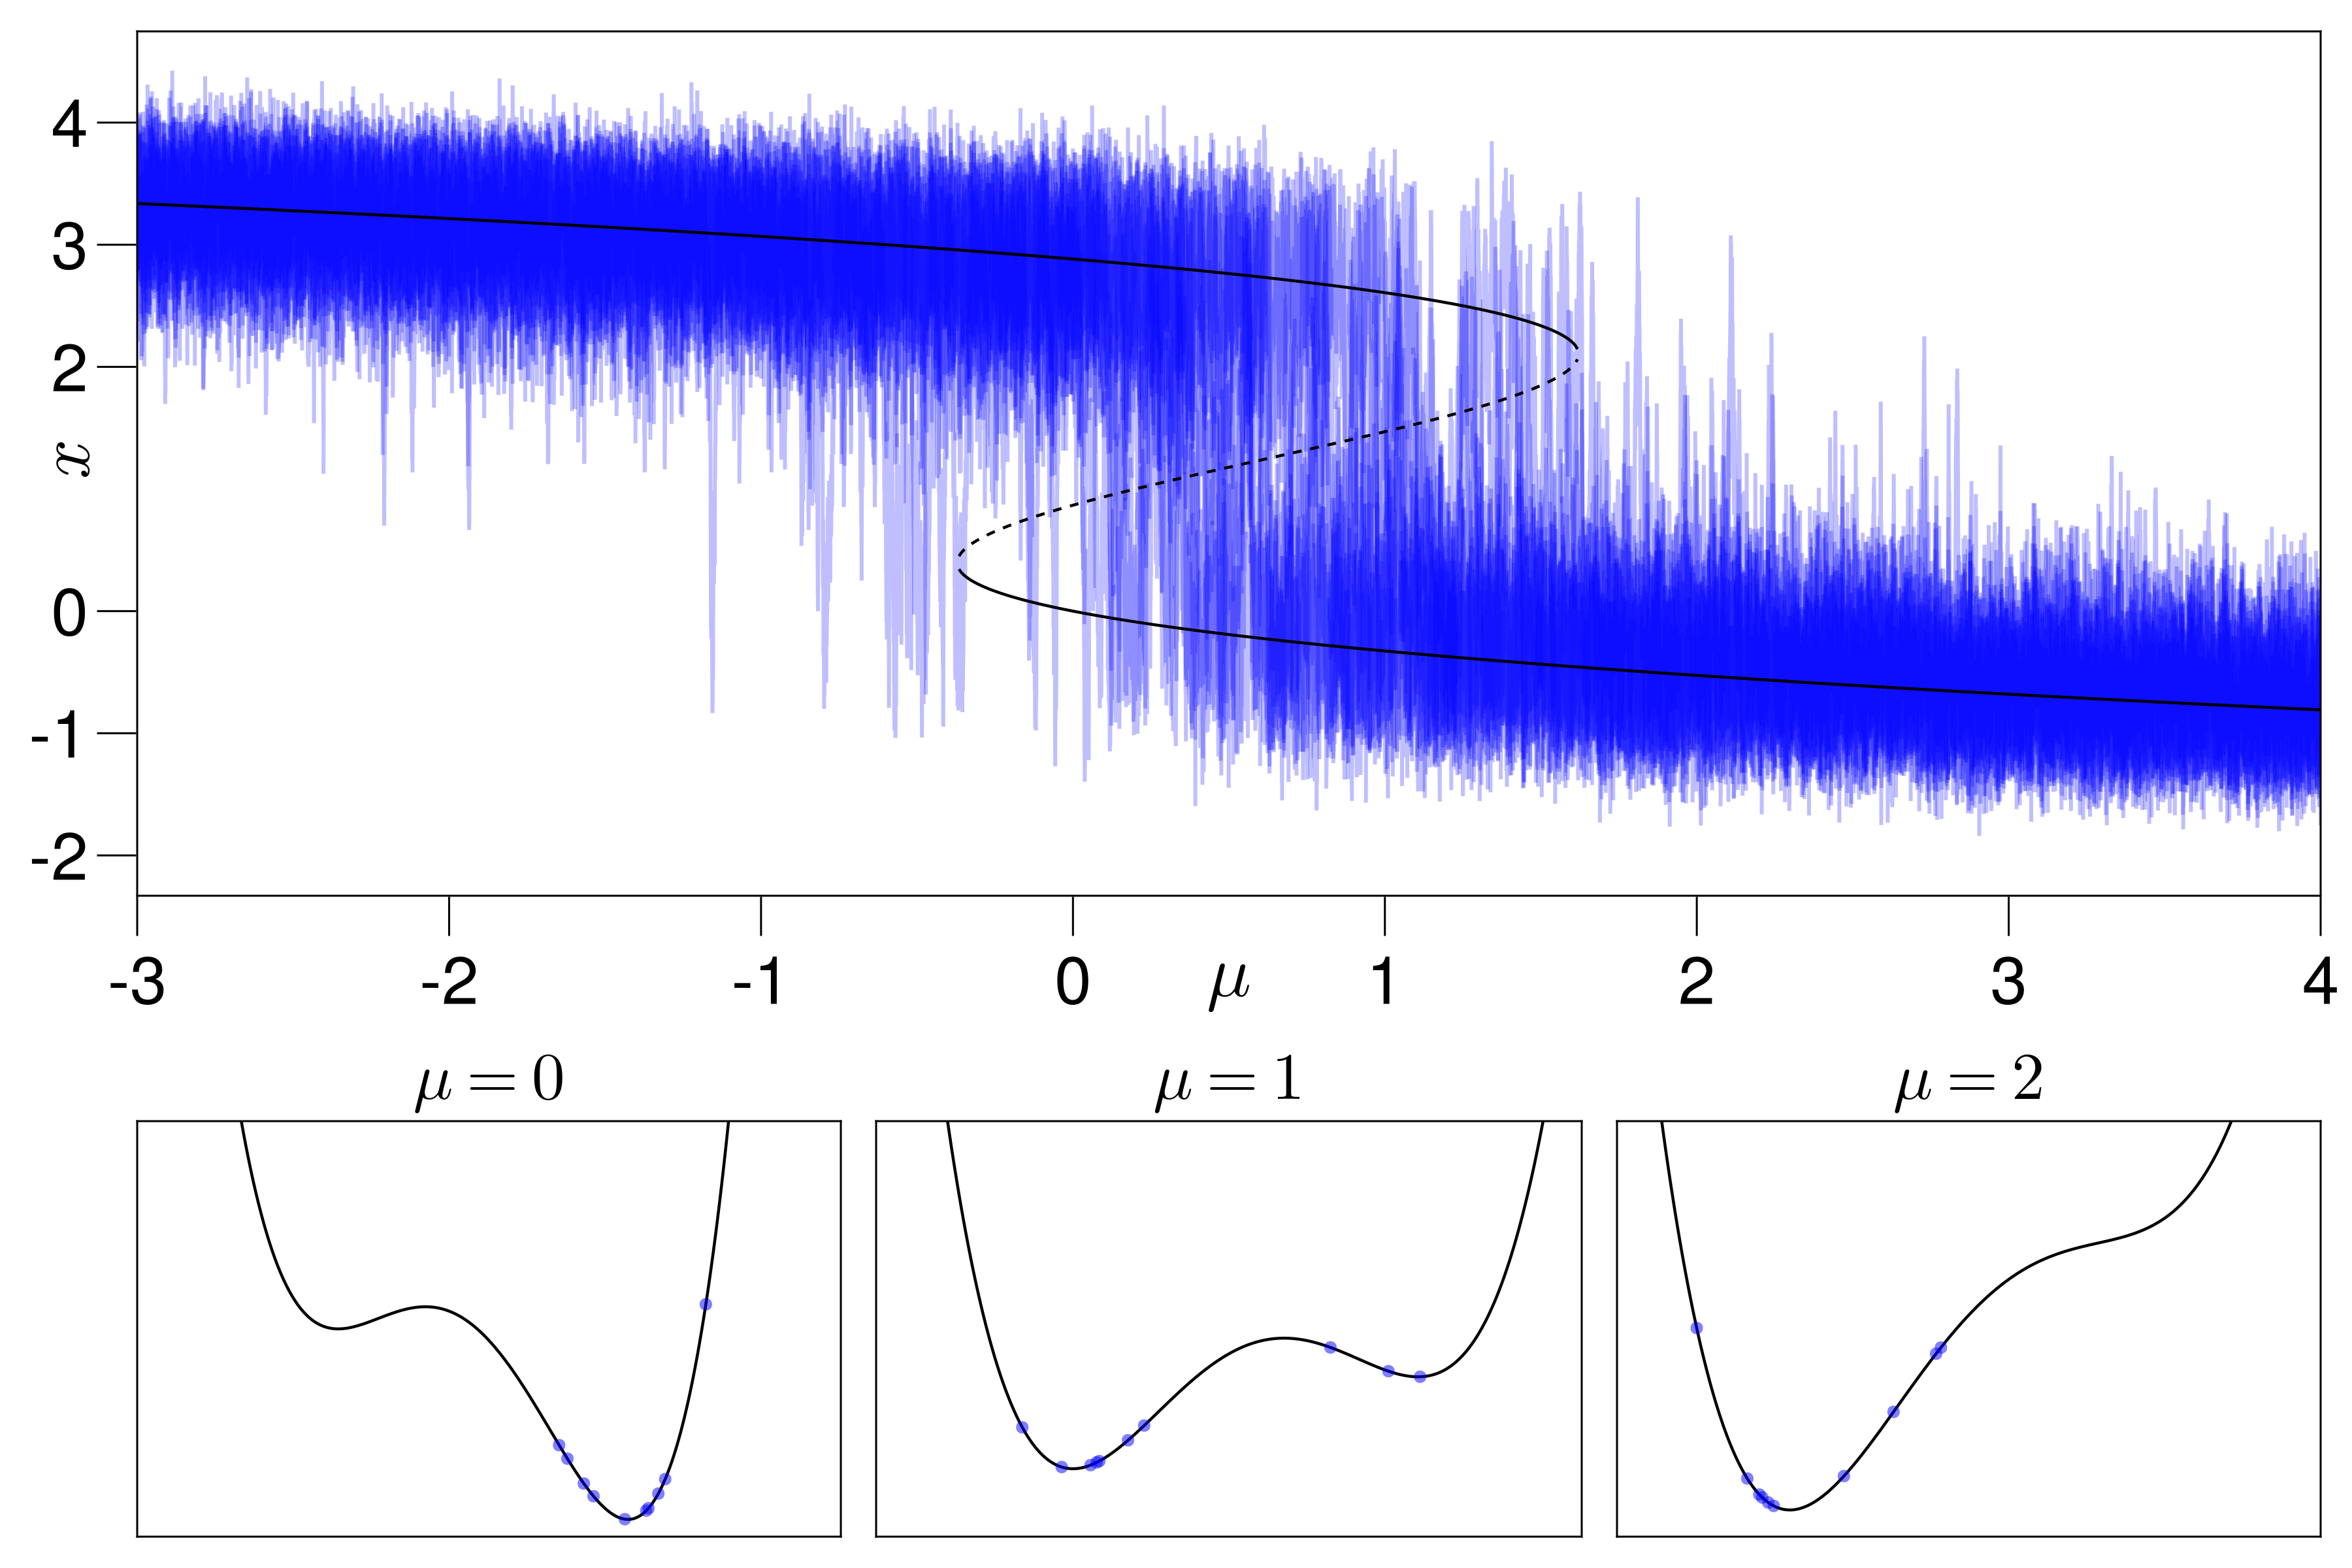
\includegraphics[keepaspectratio, width = \linewidth]{../figures/fig1.3.2.png}
        \caption{}
        \label{fig1.3.2}
   \end{subfigure}
    \caption{Ensemble sample paths of a bistable saddle-node bifurcation in low-noise (a) and highly stochastic (b) regimes. 
    The potential function is displayed in the bottom panels at parameter values $\mu=0,1$ in the bistability region and $\mu=2$ past the bifurcation; distribution of the ensemble states are plotted as dots on the potential function. 
We can clearly see how the high noise levels in (b) causes flickering anticipating substantially the critical threshold and this results in the ensemble states being considerably less clustered in the potential minima w.r.t. the low-noise case in (a). Details on the system and the potential function are provided in the Supplementary material.}
    \label{fig1.3}
\end{figure}
The newly introduced precursor, by its very nature, complicated the analysis of the dynamics far from the bifurcation since high level of noise may cause the system to switch back and forth between alternative stable states and, as previously established, the prediction of these noise-induced tipping is considerably harder than those that are associated to bifurcations. 
In 2012 the influence of \textit{strong noise} in a multi-decadal lake eutrophication experiment showed that skewness and autocorrelation display opposite trends w.r.t. the increase in variance \cite{Wang12} which led to the conclusion that the latter could have only be caused by flickering rather than CSD.
The meaningful consequence of this is that, in \textit{``highly stochastic dynamics"}, the switch to bistable regimes sets in quite earlier than CSD (see Figure \ref{fig1.3}), i.e. when the alternative attractor becomes strong enough such that the noise-induced fluctuations will cause excursions across the entire basin of attraction.
Further evidence of this was given one year later by Dakos, van Nes and Scheffer \cite{Dakos13} which systematically registered increase in variance and decrease of autocorrelation (symptomatic of flickering) in highly noisy but low-resolution timeseries well ahead of the CSD associated to a saddle-node bifurcation.
While all these results firmly placed skewness as an indicator of flickering, the increase in variance was now linked to both CSD and flickering depending on the noise-level embedded in the realizations of the stochastic process and the size shrinking of the basin of attraction in a multistable regime.
The underlying implication is that it would not always be possible to rely on timeseries data alone to distinguish between the two different drivers of critical transitions given the low dimensionality of the model, by which we mean that the mere observation of the temporal realizations of the stochastic processes will forcibly discard potentially useful information that could otherwise help to determine robustly the distance from upcoming thresholds.
As such, other works were starting to address the possibility of including spatial dependence in their models in the hope of enriching the forewarning capability of EWS.
\subsubsection{Investigation of spatially extended systems}\label{subsubsec1.2.4}
The first evidence of accounting spatial information in the context of critical transitions is from the 1998 series of works by Gandhi and colleagues \cite{Gandhi98} which realised that, whenever the dynamics of competing species are dominated by spatial clusters (as opposed to the usual assumption of well-mixing of the population densities) proxies of CSD marking the distance to extinction can be determined s.a. the correlation length (average cluster size). 
These works also noted that spatial aggregation through mean-field approximation (MFA) averages out the fluctuations that become dominant as the phase transition is approached thereby providing some insights on the loss of information when space is not accounted in dynamical models.
\paragraph{2000s}
Some years later in 2004, the MFA of well-mixed ecosystems with bistable regimes was again called into question when considering natural catastrophic shifts that feature the emergence of self-organising patches of consumers and resources \cite{Rietkerk04}, s.a. those found in arid and savanna vegetation patterns. 
This called for the extension to spatial domains to recognise self-organised patchiness as a precursor of regime shifts.
One year later, self-organised patchiness (equivalently known as pattern-formation or Turing instability) was again suggested as a forerunner of catastrophic shifts for asthma attacks \cite{Venegas05}. 
It compared experimental evidence via positron emission tomography (PET) of cluster ventilation defects (CVDs) in the lung with the effect of spatial heterogeneity breaking the uniform smooth muscle activation in a computational model of a symmetric bronchial tree. 
It was observed specifically how the local bistability of the airway tree induces the patchy self-organisation of CVDs. 
Further evidence of spatial patterns preluding ecosystem collapses was presented in 2007 when it was observed that the size distribution of the vegetation patches in Mediterranean arid environments (found in Souther Spain, Greece and North-Western Morocco) follows a power law with the number of such patches prior to desertification \cite{Kefi07}. 
As it became increasingly clear that pattern-formation was yet another form of precursor capturing the insofar neglected spatial information, a consistent statistical measure of such a phenomenon was still lacking.
In 2009 Guttal et al. \cite{Guttal09} put a remedy to this deficiency by introducing spatial variance and spatial skewness as a first form of leading indicators. 
In particular they show how an increase in the former and changes in the latter provide clear indications of pattern-forming transitions to bistablity regimes in a spatially extended population model.
Furthermore it was demonstrated how these two indicators can overcome the limitations imposed by low temporal resolution of the timeseries of the MFA of the model.
\paragraph{Mid 2010s}
The 2010s thus marked the beginning of the analysis of spatio-temporal EWS, particularly by the ecologists.
Carpenter and Brock \cite{Carpenter10} used the discrete Fourier transform (DFT) to extend the previously conceived concept of spectral reddening of a timeseries experiencing CSD \cite{Kleinen03} to shifts to lower spatial frequencies for period-doubling (Ricker map) and bistable (predator-prey and harvester-prey) transitions in $4$ ecological models.
Concurrently Dakos, van Nes, Scheffer et al. \cite{Dakos10} proposed spatial correlation as the leading indicator of CSD prior to the bifurcations in overharvesting, eutrophication and vegetation turbidity reaction-diffusion models.
Specifically they compared the signal provided by Moran's two-points correlation coefficient (used to calculate the spatial correlation of neighboring cells in a $2-$dimensional lattice) with that of the temporal autocorrelation at lag$-1$ of the spatially aggregated model and found that the former consistently outperforms the latter.
In 2011 the aforementioned authors and others \cite{Dakos11} applied the same ideas to spatially-patterned vegetation changes at the onset of desertification and concluded that CSD was not detected by rising temporal variance and autocorrelation as opposed to their spatial counterparts which were able to show positive trends leading to both CSD and Turing instabilities.
Experimental evidence from a whole-ecosystem food-web monitoring of predators' distribution in a lake \cite{Cline14} also indicated that spatial variance and shifts to low spatial frequencies using the DFT provided EWS for the emergence of prey fish patchiness one year in advance of the bistable transition in the populations.
\paragraph{Late 2010s and 2020s}
Nevertheless, pattern-formation is only one of the many dynamical phenomena that affect the stability of spatio-temporal systems (as we will explore in the third Chapter of the present work). 
In fact Kuehn et al. in 2013 \cite{Kuehn13} and Leemput, van Nes and Scheffer in 2015 \cite{Leemput15} indipendently considered travelling waves of invasion fronts connecting two well-separated initial populations distributions. They both indicated the slow-down (or \textit{pinning}) of the wavespeed as a precursor to the critical point at which the resilience of two alternative stable states of high and low biomass is equal (called Maxwell point).
Investigation of spatio-temporal EWS also extended to nework-based analysis in the later part of the decade with the maximum element of the covariance matrix \cite{Suweis14}, the noise-dependent characteristic return time of a dimensionality reduction of a coupled network \cite{Liang17}, the spatial correlation of a multiplex disease network \cite{Jentsch18} and the slower reovery from perturbation of mutualistic communities \cite{Lever20} all providing candidate spatial indicators.
The latest efforts of the current decade also proposed the adoption of techniques from statistical mechanics \cite{Chen19,Gottwald20,Donovan22} for spatio-temporal systems as well as deep-learning \cite{Bury21,Dylewsky23} for the automatic detection of combined signals albeit with questionable insights gained from the interpretation of their meaning. 
\end{document}
